\let\negmedspace\undefined
\let\negthickspace\undefined
\documentclass[journal,12pt,onecolumn]{IEEEtran}
\usepackage{cite}
\usepackage{amsmath,amssymb,amsfonts,amsthm}
\usepackage{algorithmic}
\usepackage{graphicx}
\usepackage{textcomp}
\usepackage{xcolor}
\usepackage{txfonts}
\usepackage{listings}
\usepackage{enumitem}
\usepackage{mathtools}
\usepackage{gensymb}
\usepackage{comment}
\usepackage[breaklinks=true]{hyperref}
\usepackage{tkz-euclide} 
\usepackage{listings}
\usepackage{gvv}                                        
%\def\inputGnumericTable{}                                 
\usepackage[utf8]{inputenc}
    \usepackage{tfrupee}
    \usepackage{newunicodechar}
\newunicodechar{₹}{\text{\rupee}}

\usepackage{xparse}
\usepackage{color}                                            
\usepackage{array}                                            
\usepackage{longtable}                                       
\usepackage{calc}                                             
\usepackage{multirow}
\usepackage{multicol}
\usepackage{hhline}                                           
\usepackage{ifthen}                                           
\usepackage{lscape}
\usepackage{tabularx}
\usepackage{array}
\usepackage{float}
\newtheorem{theorem}{Theorem}[section]
\newtheorem{problem}{Problem}
\newtheorem{proposition}{Proposition}[section]
\newtheorem{lemma}{Lemma}[section]
\newtheorem{corollary}[theorem]{Corollary}
\newtheorem{example}{Example}[section]
\newtheorem{definition}[problem]{Definition}
\newcommand{\BEQA}{\begin{eqnarray}}
\newcommand{\EEQA}{\end{eqnarray}}
\usepackage{float}
%\newcommand{\define}{\stackrel{\triangle}{=}}
\theoremstyle{remark}
\usepackage{ circuitikz }
\begin{document}

\title{2025 XE}
\author{EE25BTECH11021 - Dhanush sagar}
\maketitle
\renewcommand{\thefigure}{\theenumi}
\renewcommand{\thetable}{\theenumi}
\title{2025 Xe}
\author{Dhanush Sagar}
\date{August 2025}

\begin{enumerate}


\item Even though I had planned to go skiing with my friends, I had to \rule{3cm}{0.15mm} at the last moment because of an injury.  
Select the most appropriate option to complete the above sentence.

\hfill [GATE XE 2025]

\begin{multicols}{2}
\begin{enumerate}
\item back up
\item back of
\item back on
\item back out
\end{enumerate}
\end{multicols}

% Q2
\item The President, along with the Council of Ministers, \rule{3cm}{0.15mm} to visit India next week.  
Select the most appropriate option to complete the above sentence.

\hfill [GATE XE 2025]

\begin{multicols}{2}
\begin{enumerate}
\item wish
\item wishes
\item will wish
\item is wishing
\end{enumerate}
\end{multicols}

% Q3
\item An electricity utility company charges ₹ 7 per kWh (kilo watt-hour). If a 40-watt desk light is left on for 10 hours each night for 180 days, what would be the cost of energy consumption? If the desk light is on for 2 more hours each night for the 180 days, what would be the percentage-increase in the cost of energy consumption?

\hfill [GATE XE 2025]

\begin{multicols}{2}
\begin{enumerate}
\item ₹ 604.8; 10\%
\item ₹ 504; 20\%
\item ₹ 604.8; 12\%
\item ₹ 720; 15\%
\end{enumerate}
\end{multicols}

% Q4
\item In the context of the given figure, which one of the following options correctly represents the entries in the blocks labelled (i), (ii), (iii), and (iv), respectively?
\begin{figure}[H]
    \centering
    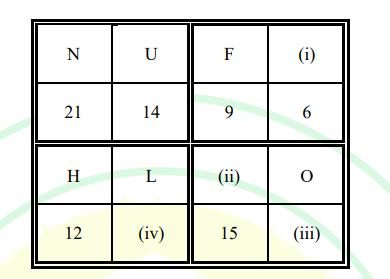
\includegraphics[width=0.5\columnwidth]{figs/fig1.png}
    \caption{}
    \label{fig:placeholder}
    
\end{figure}
\hfill [GATE XE 2025]

\begin{multicols}{2}
\begin{enumerate}
\item Q, M, 12, and 8
\item K, L, 10, and 14
\item I, J, 10, and 8
\item L, K, 12, and 8
\end{enumerate}
\end{multicols}

% Q5
\item A bag contains Violet (V), Yellow (Y), Red (R), and Green (G) balls. On counting them, the following results are obtained:  

(i) The sum of Yellow balls and twice the number of Violet balls is 50.  \\
(ii) The sum of Violet and Green balls is 50.  \\
(iii) The sum of Yellow and Red balls is 50.  \\
(iv) The sum of Violet and twice the number of Red balls is 50. \\ 



Which one of the following Pie charts correctly represents the balls in the bag?

\hfill [GATE XE 2025]

\begin{figure}[H]
    \centering
    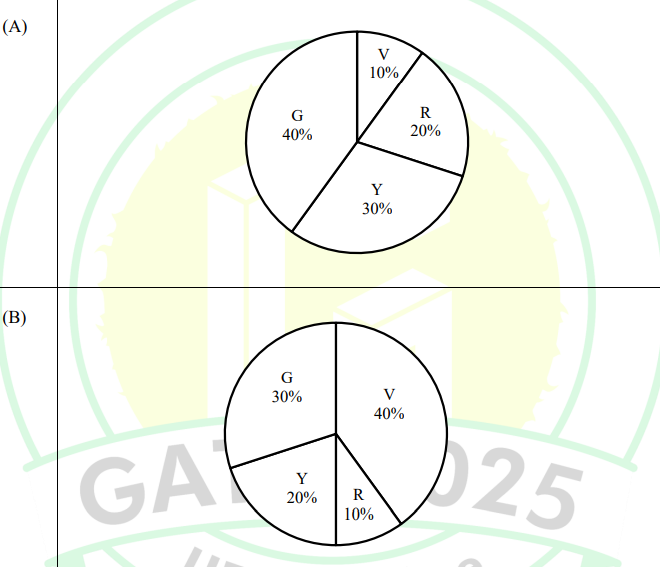
\includegraphics[width=0.4\columnwidth]{figs/fig2.png}
    \caption{}
    \label{fig:placeholder}
\end{figure}

\begin{figure}[H]
    \centering
    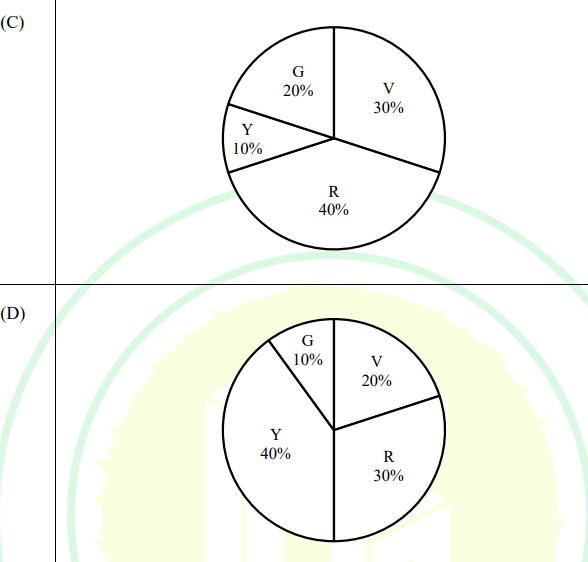
\includegraphics[width=0.4\columnwidth]{figs/fig3.png}
    \caption{}
    \label{fig:placeholder}
\end{figure}

% Q6
\item “His life was divided between the books, his friends, and long walks. A solitary man, he worked at all hours without much method, and probably courted his fatal illness in this way. To his own name there is not much to show; but such was his liberality that he was continually helping others, and fruits of his erudition are widely scattered, and have gone to increase many a comparative stranger’s reputation.”  
(From E.V. Lucas’s “A Funeral”)  

Based only on the information provided in the above passage, which one of the following statements is true?

\hfill [GATE XE 2025]

\begin{multicols}{2}
\begin{enumerate}
\item The solitary man described in the passage is dead.
\item Strangers helped create a grand reputation for the solitary man.
\item The solitary man described in the passage found joy in scattering fruits.
\item The solitary man worked in a court where he fell ill.
\end{enumerate}
\end{multicols}

% Q7
\item For the clock shown in the figure, if  
$O^* = OQSZPRT$ and $X^* = XZPWYOQ$, then which one among the given options is most appropriate for $P^*$?



\begin{figure}[H]
    \centering
    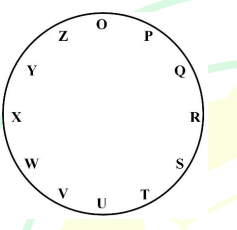
\includegraphics[width=0.5\columnwidth]{figs/fig4.png}
    \caption{}
    \label{fig:placeholder}
\end{figure}

\hfill [GATE XE 2025]

\begin{multicols}{2}
\begin{enumerate}
\item $P \ U \ W \ R \ T \ V \ X$
\item $P \ R \ T \ O \ Q \ S \ U$
\item $P \ T \ V \ Q \ S \ U \ W$
\item $P \ S \ U \ P \ R \ T \ V$
\end{enumerate}
\end{multicols}

% Q8
\item Consider a five-digit number $PQRST$ that has distinct digits $P, Q, R, S,$ and $T$, and satisfies the following conditions:  
$P < Q$, $S > P > T$, $R < T$.  

If integers 1 through 5 are used to construct such a number, the value of $P$ is:

\hfill [GATE XE 2025]

\begin{multicols}{2}
\begin{enumerate}
\item 1
\item 2
\item 3
\item 4
\end{enumerate}
\end{multicols}

% Q9
\item A business person buys potatoes of two different varieties P and Q, mixes them in a certain ratio and sells them at ₹192 per kg.  
The cost of the variety P is ₹800 for 5 kg.  
The cost of the variety Q is ₹800 for 4 kg.  
If the person gets 8\% profit, what is the P:Q ratio (by weight)?

\hfill [GATE XE 2025]

\begin{multicols}{2}
\begin{enumerate}
\item 5:4
\item 3:4
\item 3:2
\item 1:1
\end{enumerate}
\end{multicols}

% Q10
\item Three villages P, Q, and R are located in such a way that the distance $PQ = 13$ km, $QR = 14$ km, and $RP = 15$ km, as shown in the figure.  
A straight road joins Q and R. It is proposed to connect P to this road QR by constructing another road.  
What is the minimum possible length (in km) of this connecting road?

\begin{figure}[H]
    \centering
    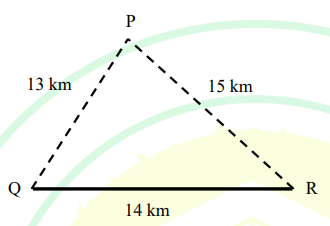
\includegraphics[width=0.5\columnwidth]{figs/fig5.png}
    \caption{}
    \label{fig:placeholder}
\end{figure}

\hfill [GATE XE 2025]

\begin{multicols}{2}
\begin{enumerate}
\item 10.5
\item 11.0
\item 12.0
\item 12.5
\end{enumerate}
\end{multicols}

\item Let $X$ and $Y$ be two random variables with mean $0$, variance $1$, and correlation coefficient $\tfrac{1}{3}$.  
Then the value of $\text{Var}(X+3Y)$ is equal to

\hfill [GATE XE 2025]

\begin{multicols}{2}
\begin{enumerate}
\item 9
\item 10
\item 11
\item 12
\end{enumerate}
\end{multicols}

% Q12
\item Consider the second order Partial Differential Equation (PDE)  
\begin{align}
    4x^2 \frac{\partial^2 u}{\partial x^2} + 4(x+y)\frac{\partial^2 u}{\partial x \partial y} + (x^2+y^2)\frac{\partial^2 u}{\partial y^2} - u = 0
\end{align} 
Then which one of the following statements is correct?

\hfill [GATE XE 2025]

\begin{multicols}{2}
\begin{enumerate}
\item The PDE is hyperbolic in the region $\{(x,y)\in\mathbb{R}^2 : -1 < x < 0, \ y < 0\}$
\item The PDE is hyperbolic in the region $\{(x,y)\in\mathbb{R}^2 : 1 < x < \infty, \ y < 0\}$
\item The PDE is elliptic in the region $\{(x,y)\in\mathbb{R}^2 : 0 < x < 1, \ y > 0\}$
\item The PDE is parabolic in the region $\{(x,y)\in\mathbb{R}^2 : 1 < x < \infty, \ y < 0\}$
\end{enumerate}
\end{multicols}

% Q13
\item Consider the infinite series  
\begin{align}
    (P): \sum_{n=2}^{\infty} \frac{1}{(n \log n)^{1/n}},  (Q): \sum_{n=1}^{\infty} \frac{n^n}{(2n)!}
\end{align}
Then which one of the following statements is correct?

\hfill [GATE XE 2025]

\begin{multicols}{2}
\begin{enumerate}
\item Series $(P)$ and $(Q)$ both converge
\item Series $(P)$ converges and series $(Q)$ diverges
\item Series $(P)$ and $(Q)$ both diverge
\item Series $(P)$ diverges and series $(Q)$ converges
\end{enumerate}
\end{multicols}

% Q14
\item Suppose the polynomial $a+bx+cx^2+dx^3$ interpolates the data $(-1,1), (0,3), (1,2), (2,4)$.  
Then which one of the following statements is correct?

\hfill [GATE XE 2025]

\begin{multicols}{2}
\begin{enumerate}
\item $a=-2c,\ d=-2b$
\item $a=2c,\ d=2b$
\item $b=3c,\ a=2d$
\item $b=2c,\ a=3d$
\end{enumerate}
\end{multicols}

% Q15
\item Let $C$ be the positively oriented boundary of the domain bounded by the curves $y=2x^2$ and $y^2=4x$.  
Then the value of the line integral  
\begin{align}
    \oint_C (2y^2+2xy+4y)\,dx + (x^2+4xy+8x)\,dy
\end{align} 
is equal to

\hfill [GATE XE 2025]

\begin{multicols}{2}
\begin{enumerate}
\item $\tfrac{8}{3}$
\item $\tfrac{2}{3}$
\item $\tfrac{4}{3}$
\item $\tfrac{1}{3}$
\end{enumerate}
\end{multicols}

% Q16
\item Let $y(x)$ be the solution of the initial value problem  
\begin{align}
    x^2y''+xy'-y=0, x>0, y(1)=0,\ y'(1)=2.
\end{align}
Then the value of $y'\brak{\tfrac{1}{2}}$ is equal to (Answer in integer) \rule{3cm}{0.15mm}.

\hfill [GATE XE 2025]

% Q17
\item Suppose that $2$ is an eigenvalue of the matrix  
\begin{align}
    \myvec{0 & 3 & -\alpha \\ 0 & 1 & 0 \\ 1 & -1 & 3}
\end{align}  
Then the value of $\alpha$ is equal to (Answer in integer) \rule{3cm}{0.15mm}.

\hfill [GATE XE 2025]

% Q18
\item Let $f(z)$ be an analytic function such that $\Re(f'(z)) = 3x^2-4y-3y^2$, $f(i)=0$, $f'(0)=0$, where $i=\sqrt{-1}$.  
Then the value of $f(1)$ is equal to

\hfill [GATE XE 2025]

\begin{multicols}{2}
\begin{enumerate}
\item $4+2i$
\item $1+5i$
\item $1-i$
\item $4-2i$
\end{enumerate}
\end{multicols}

% Q19
\item Consider the function $f(x,y) = x^2y + 2xy^2 - 2x^2y^2$.  
Then which one of the following statements is correct?

\hfill [GATE XE 2025]

\begin{multicols}{2}
\begin{enumerate}
\item $\brak{\tfrac{3}{2},0}$ is a point of local maxima of $f$
\item $\brak{0,\tfrac{3}{4}}$ is a point of local minima of $f$
\item $\brak{\tfrac{3}{2},\tfrac{3}{4}}$ is a point of local maxima of $f$
\item $\brak{\tfrac{3}{2},\tfrac{3}{4}}$ is a saddle point of $f$
\end{enumerate}
\end{multicols}

% Q20
\item For $a,b \in \mathbb{R}$, consider the system of linear equations:  
\begin{align}
x+y+az=2,  2y+2z=1,  ax+2z=b
\end{align}  
If the system has infinitely many solutions, then which of the following statements is/are correct?

\hfill [GATE XE 2025]

\begin{multicols}{2}
\begin{enumerate}
\item $a=2,\ b=3$
\item $a=2,\ b=5$
\item $a=-1,\ b=-\tfrac{3}{2}$
\item $a=3,\ b=5$
\end{enumerate}
\end{multicols}

% Q21
\item Let $u(x,t)$ be the solution of the initial boundary value problem  
\begin{align}
\frac{\partial u}{\partial t} - \frac{\partial^2 u}{\partial x^2} - u = 0,  0<x<\pi,\ t>0
\end{align}  
\begin{align}
u(x,0)=2\sin\brak{\tfrac{3x}{2}}\cos\brak{\tfrac{x}{2}}, u(0,t)=u(\pi,t)=0, \ t>0
\end{align}  
Then the value of $\lim_{t\to\infty} u\brak{\tfrac{3\pi}{4},t}$ is equal to (rounded off to two decimal places) \rule{3cm}{0.15mm}.

\hfill [GATE XE 2025]



\item Fluid at a constant flow rate passes through a long, straight, cylindrical pipe that has an axisymmetric convergent section at the end. Which one of the following options correctly represents the velocity field in the converging section in cylindrical $(r,\theta,z)$ coordinates? \label{q:22}

\hfill[GATE XE 2025]

\begin{multicols}{2}
\begin{enumerate}
\item Two-dimensional function of $r$ and $z$
\item One-dimensional function of $r$
\item Two-dimensional function of $r$ and $\theta$
\item One-dimensional function of $z$
\end{enumerate}
\end{multicols}


\item A sharp flat plate of length $L$ and infinite width is immersed parallel to a fluid stream having velocity $u_\infty$. At a point on the plate, far away from the leading edge and not near the trailing edge, the boundary layer thickness, the displacement thickness, and the momentum thickness are denoted as $\delta$, $\delta^*$, and $\theta$, respectively. Which one of the following options correctly represents the relation between these thicknesses? \label{q:23}

\hfill[GATE XE 2025]

\begin{multicols}{2}
\begin{enumerate}
\item $\delta > \delta^* > \theta$
\item $\delta > \theta > \delta^*$
\item $\delta^* > \delta > \theta$
\item $\theta > \delta^* > \delta$
\end{enumerate}
\end{multicols}


\item Consider the following Statements [1] and [2]. \\
Statement [1]: The Eulerian study focusses attention on individual particle and its motion is observed as a function of time. \\
Statement [2]: The Lagrangian study focusses attention on the motion of the particles passing through an identified point. \\
Which one of the following options identifies the correctness of the given statements? \label{q:24}

\hfill[GATE XE 2025]

\begin{multicols}{2}
\begin{enumerate}
\item Both [1] and [2] are correct.
\item Both [1] and [2] are NOT correct.
\item [1] is correct, but [2] is NOT correct.
\item [1] is NOT correct, but [2] is correct.
\end{enumerate}
\end{multicols}


\item Statement of Reynolds Transport Theorem is given below with three blanks. \\
The rate of change of \rule{3cm}{0.15mm} extensive property can be calculated by summing the rate of change of the amount of same property in the \rule{3cm}{0.15mm} and the rate at which the property is \rule{3cm}{0.15mm} the surface of the control volume. \\
Which one of the following options correctly fills the blanks by using its comma-separated phrases in sequence? \label{q:25}

\hfill[GATE XE 2025]

\begin{multicols}{2}
\begin{enumerate}
\item system, control volume, exiting
\item control volume, system, exiting
\item system, control volume, entering
\item control volume, control volume, entering
\end{enumerate}
\end{multicols}


\item For a steady and incompressible flow, the velocity field ($\vec{V}$) in Cartesian $(x,y,z)$ coordinate system is given as: $\vec{V}=5x\,\hat{\imath}-Py\,\hat{\jmath}+3\,\hat{k}$. Here, $\hat{\imath}$, $\hat{\jmath}$, and $\hat{k}$ are unit vectors along $x$, $y$, and $z$ directions, respectively and $P$ is a constant. Which one of the following options is the correct value of $P$ that satisfies the conservation of mass for the given velocity field? \label{q:26}

\hfill[GATE XE 2025]

\begin{multicols}{2}
\begin{enumerate}
\item 5
\item $-5$
\item 8
\item 2
\end{enumerate}
\end{multicols}


\item Conservation of mass for a steady axisymmetric flow field in the cylindrical $(r,z)$ coordinates is:
\begin{align}
\frac{1}{r}\frac{\partial (rV_r)}{\partial r}+\frac{\partial V_z}{\partial z}=0
\end{align}
Here, $V_r$ and $V_z$ are radial and axial components of velocity, respectively. Which one of the following options is correct if $\psi$ is the stream function? \label{q:27}

\hfill[GATE XE 2025]

\begin{multicols}{2}
\begin{enumerate}
\item $V_r=\dfrac{\partial \psi}{\partial z}$ and $V_z=-\dfrac{1}{r}\dfrac{\partial \psi}{\partial r}$
\item $V_r=\dfrac{1}{r}\dfrac{\partial \psi}{\partial z}$ and $V_z=-\dfrac{1}{r}\dfrac{\partial \psi}{\partial r}$
\item $V_r=\dfrac{1}{r}\dfrac{\partial \psi}{\partial z}$ and $V_z=\dfrac{1}{r}\dfrac{\partial \psi}{\partial r}$
\item $V_r=\dfrac{1}{r}\dfrac{\partial \psi}{\partial z}$ and $V_z=-\dfrac{\partial \psi}{\partial r}$
\end{enumerate}
\end{multicols}


\item Group-I indicates different properties of fluid and Group-II defines their basic dimensions in terms of Force $(F)$, Length $(L)$, and Time $(T)$. \\
\begin{center}
\begin{tabular}{|c|l|c|l|}
\hline
\textbf{Group-I} & & \textbf{Group-II} & \\
\hline
P & Dynamic viscosity & 1 & $FL^{-4}T^2$ \\
Q & Surface tension    & 2 & $FL^{-2}T$ \\
R & Density            & 3 & $FL^{-1}$ \\
\hline
\end{tabular}
\end{center}

\hfill[GATE XE 2025]

\begin{multicols}{2}
\begin{enumerate}
\item P–1, Q–3, R–2
\item P–2, Q–1, R–3
\item P–3, Q–2, R–1
\item P–2, Q–3, R–1
\end{enumerate}
\end{multicols}


\item Consider the steady, incompressible, and fully developed laminar flow of a fluid through a circular pipe. Here, $\Delta P$ is the pressure drop in the direction of the flow and $V$ is the average axial velocity of the fluid at any cross-section. The relation between $\Delta P$ and $V$ is: $\Delta P=K V^n$ where $K$ and $n$ are constants. Which one of the following options is the correct value of $n$? \label{q:29}

\hfill[GATE XE 2025]

\begin{multicols}{2}
\begin{enumerate}
\item 1
\item 2
\item 1.75
\item 0.5
\end{enumerate}
\end{multicols}


\item A doublet is the resulting flow pattern when a sink and a source of equal strength are brought together. Which one of the following options correctly represents the nature of the product of the strength and the distance between them during approach? \label{q:30}

\hfill[GATE XE 2025]

\begin{multicols}{2}
\begin{enumerate}
\item Remains always constant
\item Continuously decreases
\item Continuously increases
\item First increases and then continuously decreases after reaching a maximum
\end{enumerate}
\end{multicols}


\item Figure shows two parallel plates (upper plate at $x=b$ and lower one at $x=-b$) of length $L$ (aligned in $z$ direction) and infinite width (in $y$ direction, normal to the plane of the figure). Two immiscible, incompressible liquids are flowing steadily in the $z$ direction through the thin passage between the plates under the influence of horizontal pressure gradient $(P_0-P_L)/L$. During the flow, the passage is always half-filled with denser fluid I (viscosity $\mu_I$) at the bottom and rest is occupied by lighter fluid II (viscosity $\mu_{II}$; $\mu_{II}<\mu_I$). Considering exactly planar interface between the fluids and no instabilities in the flow, the shear stress, $\tau_{xz}$ is expressed as:
\begin{align}
\tau_{xz}=\frac{(P_0-P_L)b}{L}\left[\brak{\frac{x}{b}}-\frac{1}{2}\brak{\frac{\mu_I-\mu_{II}}{\mu_I+\mu_{II}}}\right]
\end{align}
Which one of the following options correctly identifies the location of the point having maximum velocity of the flow? \label{q:31}

\begin{figure}[H]
    \centering
    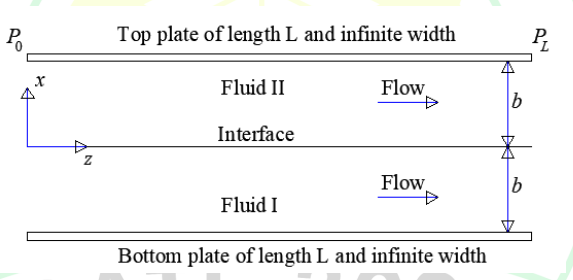
\includegraphics[width=0.5\columnwidth]{figs/fig6.png}
    \caption{}
    \label{fig:placeholder}
\end{figure}


\hfill[GATE XE 2025]

\begin{multicols}{2}
\begin{enumerate}
\item Above the interface
\item Below the interface
\item At the interface
\item At the top plate
\end{enumerate}
\end{multicols}


\item Group-I shows different two-dimensional bodies and Group-II mentions their total drag coefficient $(C_D)$ based on frontal area while facing parallel flow of fluid having Reynolds number $Re\ge 10^4$ along the direction of arrow. The bodies are placed symmetrically with respect to the flow direction. \\
\begin{figure}[H]
    \centering
    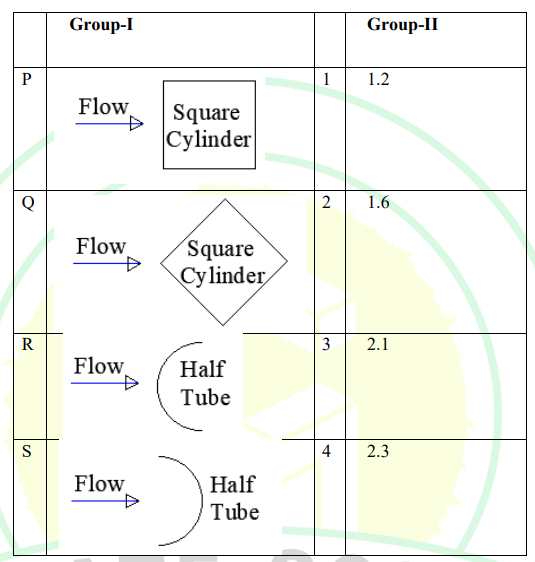
\includegraphics[width=0.5\columnwidth]{figs/fig7.png}
    \caption{}
    \label{fig:placeholder}
\end{figure}

Which one of the following options identifies the correct match between Group-I and Group-II, as per the concept of degree of streamlining? \label{q:32}


\hfill[GATE XE 2025]

\begin{multicols}{2}
\begin{enumerate}
\item P–3, Q–2, R–1, S–4
\item P–3, Q–2, R–4, S–1
\item P–2, Q–3, R–1, S–4
\item P–3, Q–1, R–2, S–4
\end{enumerate}
\end{multicols}


\item A solid body of uniform specific gravity floats in a deep liquid pool. Take $B$, $G$, and $M$ as the centre of buoyancy, centre of gravity, and metacentre of the body, respectively. Which one of the following options is correct for the stable floatation of the body in the pool when the body is given a small tilt angle? \label{q:33}

\hfill[GATE XE 2025]

\begin{multicols}{2}
\begin{enumerate}
\item $\overline{MG}$ is the metacentric height and $G$ should lie below $M$
\item $\overline{MG}$ is the metacentric height and $B$ should lie above $M$
\item $\overline{MB}$ is the metacentric height and $B$ should lie below $M$
\item $\overline{MB}$ is the metacentric height and $G$ should lie above $M$
\end{enumerate}
\end{multicols}


\item Figure shows the steady and incompressible flow of a fluid in the direction of arrow from section A to section D. Three pipe connectors are to be placed between sections at A and D having Total Energy Line (TEL) and Hydraulic Grade Line (HGL) as depicted in the figure. Consider, $g$, $P$, $Q$, $V$, $\gamma$, and $Z$ denote gravitational acceleration, pressure, volume flow rate, velocity, specific weight, and elevation of centerline of the pipe connectors from the datum, respectively. Which one of the following options, in sequence, indicates the correct nature of connectors between sections A and B, B and C, and C and D in the direction of flow? \label{q:34}

\begin{figure}[H]
    \centering
    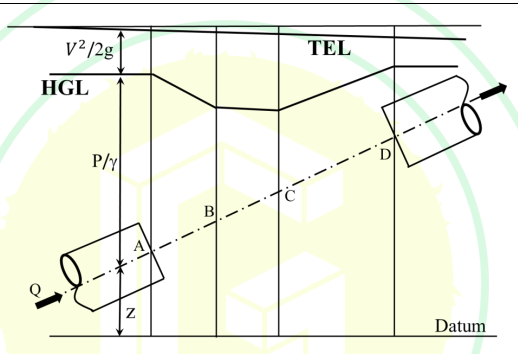
\includegraphics[width=0.5\columnwidth]{figs/fig8.png}
    \caption{}
    \label{fig:placeholder}
\end{figure}


\hfill[GATE XE 2025]

\begin{multicols}{2}
\begin{enumerate}
\item Converging, Constant area, Diverging
\item Diverging, Constant area, Converging
\item Constant area, Constant area, Constant area
\item Constant area, Converging, Diverging
\end{enumerate}
\end{multicols}


\item A liquid flows under steady and incompressible flow conditions from station 1 to station 4 through pipe sections P, Q, R, and S as shown in figure. Consider, $d$, $V$, and $h$ represent the diameter, velocity, and head loss, respectively, in each pipe section with subscripts ‘P’, ‘Q’, ‘R’, and ‘S’. $\Delta h$ represents the head difference between the inlet (station 1) and outlet (station 4). All the pipe sections are placed on the same horizontal plane for which the figure shows the top view. Which one of the following options is correct for the given flow loop? \label{q:35}

\begin{figure}[H]
    \centering
    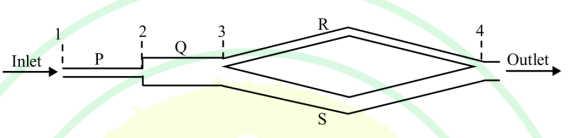
\includegraphics[width=0.5\columnwidth]{figs/fig9.png}
    \caption{}
    \label{fig:placeholder}
\end{figure}


\hfill[GATE XE 2025]


\begin{enumerate}
\item $\Delta h=h_P+h_Q+h_R+h_S$ and $V_P d_P^2=V_Q d_Q^2=V_R d_R^2=V_S d_S^2$
\item $\Delta h=h_P+h_Q+h_R$ and $V_P d_P^2=V_Q d_Q^2=V_R d_R^2=V_S d_S^2$
\item $\Delta h=h_P+h_Q+h_R$ and $V_P d_P^2=V_Q d_Q^2=V_R d_R^2+V_S d_S^2$
\item $\Delta h=h_P+h_Q+h_R+h_S$ and $V_P d_P^2=V_Q d_Q^2=V_R d_R^2+V_S d_S^2$
\end{enumerate}



\item Consider, $\hat{\imath}$ and $\hat{\jmath}$ are unit vectors along $x$ and $y$ directions of a Cartesian $(x,y)$ coordinate system, respectively and $t$ is time. Temperature $(T)$ and fluid velocity $(\vec{V})$ are given for a flow field as:
\begin{align}
    T=x^2+yt+35,\\ 
    \vec{V}=(4xy)\,\hat{\imath}+(xt-2y^2)\,\hat{\jmath}.
\end{align}
The total rate of change of temperature in the flow field (in integer) for time $t=2$ at a point $(2,3)$ is \rule{3cm}{0.15mm} \label{q:36}

\hfill[GATE XE 2025]


\item Driven by a pressure gradient of $100$ kPa/m, a fluid of dynamic viscosity $0.1$ Pa.s flows between two fixed infinitely large parallel plates under steady, incompressible, and fully developed laminar conditions. The average velocity of the flow is $2$ m/s. The gap between the parallel plates in mm (rounded off to 2 decimal places) is \rule{3cm}{0.15mm} \label{q:37}

\hfill[GATE XE 2025]


\item An incompressible fluid is flowing between two infinitely large parallel plates separated by $5$ mm distance. The bottom plate is stationary and the top plate is moving at a constant velocity of $5$ mm/s in the direction parallel to the bottom plate. The flow of the fluid between the plates is steady, two-dimensional, laminar, and the variation of fluid velocity is linear between the plates. A square fluid element of $1$ mm side is considered at equal distance from both the plates in the flow field such that one of its sides is parallel to the plates. The magnitude of circulation in mm$^2$/s (in integer) along the edges of the square fluid element is \rule{3cm}{0.15mm} \label{q:38}

\hfill[GATE XE 2025]


\item Consider, a kite weighing $100$ grams as essentially a rigid flat plate making an angle $8^\circ$ with the horizontal and having a planform area of $0.045$ m$^2$ when exposed to horizontal parallel wind of $60$ km/h. The thread string of the kite makes an angle $45^\circ$ with the horizontal. A tension of $450$ grams in the thread is necessary to float the kite steadily. Take air density as $1.2$ kg/m$^3$ and gravitational acceleration as $9.81$ m/s$^2$. The lift coefficient $(C_L)$ associated with the air flow around steadily floating kite (rounded off to 2 decimal places) is \rule{3cm}{0.15mm} \label{q:39}

\hfill[GATE XE 2025]


\item A fixed control volume has four one-dimensional boundary sections (1, 2, 3, and 4). For a steady flow inside the control volume, the flow properties at each section are tabulated below: \label{q:40}

\hfill[GATE XE 2025]

\begin{tabular}{|c|c|c|c|c|c|}
\hline
Boundary Section & Type & Density (kg/m$^3$) & Surface Normal Velocity (m/s) & Cross-sectional Area (m$^2$) & Specific Energy (J/kg) \\
\hline
1 & Inlet & 1000 & 10 & 0.5 & 200 \\
\hline
2 & Inlet & 1000 & 2 & 3.0 & 50 \\
\hline
3 & Outlet & 1000 & 5 & 1.0 & 100 \\
\hline
4 & Outlet & 1000 & 4 & 1.5 & 80 \\
\hline
\end{tabular}

The rate of change of energy of the system which occupies the control volume at this instant is $E\times 10^6$ J/s. The value of $E$ (rounded off to 2 decimal places) is \rule{3cm}{0.15mm}

\hfill[GATE XE 2025]


\item A ship is to be operated in a fluid medium with kinematic viscosity $0.032\times 10^{-3}$ m$^2$/s. A one-tenth scale model of the ship is built for testing. Consider, inertia, viscous and gravity forces are dominant for the ship and its model during the operation. The required kinematic viscosity of the liquid for testing the model is $P\times 10^{-6}$ m$^2$/s. The value of $P$ (rounded off to 2 decimal places) is \rule{3cm}{0.15mm} \label{q:41}

\hfill[GATE XE 2025]


\item Water flows through a pipe of diameter 20 cm at a flow rate of 0.025 m$^3$/s. A pitot-static tube is placed at the centre of the pipe and indicates the pressure difference of 5 cm of water column. Theoretical velocity measured through pitot-static tube when multiplied with velocity coefficient $C_V$ gives the actual velocity of the flow. If the mean velocity in the pipe is 90\% of the actual velocity at the centre of the pipe and the gravitational acceleration is 10 m/s$^2$, the value of $C_V$ (rounded off to 2 decimal places) is \rule{3cm}{0.15mm} \label{q:42}

\hfill[GATE XE 2025]


\item An oil of density 870 kg/m$^3$ and viscosity 0.036 Pa.s flows through a straight pipe of 10 cm diameter and 1.5 km length at the flow rate of 250 liters per minute under the steady and incompressible flow conditions. To control the flow rate of oil, a valve is fixed at the middle of the pipe causing no change in the total length of the pipe. The total head loss measured across the two ends of the pipe is 11.60 m. Using gravitational acceleration as 10 m/s$^2$, the minor head loss contributed by the presence of the valve in m (rounded off to 2 decimal places) is \rule{3cm}{0.15mm} \label{q:43}

\hfill[GATE XE 2025]

\item The figure below shows a plane PQR in a unit cell. The Miller indices of the plane PQR is

\begin{figure}[H]
    \centering
    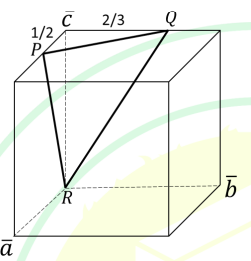
\includegraphics[width=0.5\columnwidth]{figs/fig10.png}
    \caption{}
    \label{fig:placeholder}
\end{figure}


\hfill[GATE XE 2025]

\begin{multicols}{2}
\begin{enumerate}
\item $(4\,3\,2)$
\item $(4\,3\,\bar{2})$
\item $(2\,3\,\bar{4})$
\item $(\bar{2}\,\bar{3}\,4)$
\end{enumerate}
\end{multicols}

\item The unit of measurement for magnetic dipole moment of a body is

\hfill[GATE XE 2025]

\begin{multicols}{2}
\begin{enumerate}
\item $\mathrm{A\,m^{2}}$
\item $\mathrm{A\,m^{-1}}$
\item $\mathrm{Wb\,m^{-2}}$
\item $\mathrm{Wb\,m^{2}}$
\end{enumerate}
\end{multicols}

\item $B$ is the magnetic flux density and $T_c$ is the critical temperature. The Meissner effect is represented by

\hfill[GATE XE 2025]

\begin{multicols}{2}
\begin{enumerate}
\item $B=0$ at $T\le T_c$
\item $B=0$ at $T> T_c$
\item $B\ne 0$ at $T\le T_c$
\item $\nabla B=0$ at $T=T_c$
\end{enumerate}
\end{multicols}

\item For Al–4.5 wt\% Cu alloy, the correct sequence of precipitation during age hardening at room temperature is

\hfill[GATE XE 2025]

\begin{multicols}{2}
\begin{enumerate}
\item GP zone $\to \theta'' \to \theta' \to \theta$
\item GP zone $\to \theta' \to \theta'' \to \theta$
\item GP zone $\to \theta'' \to \theta \to \theta'$
\item GP zone $\to \theta \to \theta' \to \theta''$
\end{enumerate}
\end{multicols}

\item There is NO base-centered cubic lattice among the list of 14 Bravais lattices because of one or more of the following reasons

\hfill[GATE XE 2025]

\begin{multicols}{2}
\begin{enumerate}
\item It does NOT have translational symmetry
\item It is only compatible with the symmetry of orthorhombic crystal system
\item It is only compatible with the symmetry of tetragonal crystal system
\item It does NOT have 3-fold rotation axes along the body diagonals
\end{enumerate}
\end{multicols}

\item For a conventional optical microscope, which of the following options regarding the resolution limit and the depth of field is/are correct?

\hfill[GATE XE 2025]

\begin{multicols}{2}
\begin{enumerate}
\item Resolution limit decreases with decreasing wavelength of light
\item Resolution limit decreases with decreasing refractive index of the medium
\item Depth of field decreases with increasing value of numerical aperture of the objective lens
\item Resolution limit decreases with increasing value of numerical aperture of the objective lens
\end{enumerate}
\end{multicols}

\item Which of the following phenomenon/phenomena contribute to intensity loss of electromagnetic radiation during transmission through a medium?

\hfill[GATE XE 2025]

\begin{multicols}{2}
\begin{enumerate}
\item Electronic absorption
\item Rayleigh scattering
\item Photon–phonon interaction
\item Stimulated emission
\end{enumerate}
\end{multicols}

\item If solid tin is in equilibrium with its vapor, the degree of freedom is (answer in integer) \rule{3cm}{0.15mm}

\hfill[GATE XE 2025]

\item A GaP–GaAs semiconductor LED display has a band gap of 1.9 eV. The wavelength of emitted light in $\mu$m is (rounded off to two decimal places) \rule{3cm}{0.15mm}

Given: Planck’s constant $=6.63\times 10^{-34}\ \mathrm{J\,s}$

Velocity of light $=3\times 10^{8}\ \mathrm{m\,s^{-1}}$

$1\ \mathrm{eV}=1.6\times 10^{-19}\ \mathrm{J}$

\hfill[GATE XE 2025]
\item In an FCC crystal with lattice parameter $a$, consider the reaction of two leading partial dislocations, $AB$ and $CD$, at the line of intersection of their slip planes $(111)$ and $(111\overline{1})$, respectively, as shown in the figure below. Dislocations, $AB$ and $CD$, have Burgers vectors $\vec{b}_1$ and $\vec{b}_2$, respectively, as given in the figure. Which one of the following options for the slip plane and the Burgers vector of the resulting dislocation is correct?

\begin{figure}[H]
    \centering
    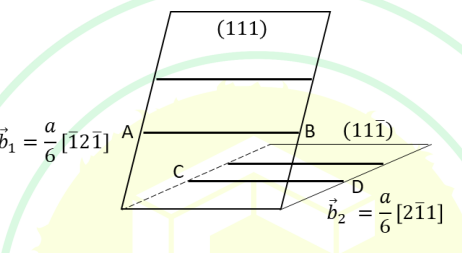
\includegraphics[width=0.5\columnwidth]{figs/fig11.png}
    \caption{}
    \label{fig:placeholder}
\end{figure}


\hfill[GATE XE 2025]

\begin{multicols}{2}
\begin{enumerate}
\item Slip plane is $(001)$ and Burgers vector is $\dfrac{a}{6}[110]$
\item Slip plane is $(11\overline{1})$ and Burgers vector is $\dfrac{a}{6}[110]$
\item Slip plane is $(001)$ and Burgers vector is $\dfrac{a}{2}[110]$
\item Slip plane is $(\overline{1}11)$ and Burgers vector is $\dfrac{a}{2}[110]$
\end{enumerate}
\end{multicols}

\item Match the detector for a scanning electron microscope (SEM) in Column I with the resulting output in Column II. \\
SE: Secondary electrons; BSE: Backscattered electrons; \\
EDS: Energy Dispersive Spectroscopy; EBSD: Electron Backscatter Diffraction

\hfill[GATE XE 2025]

\begin{center}
\begin{tabular}{l l}
\textbf{Column I} & \textbf{Column II} \\
(P) SE Detector & (1) Elemental composition analysis \\
(Q) BSE Detector & (2) Kikuchi lines \\
(R) EDS Detector & (3) Topographic image \\
(S) EBSD Detector & (4) Compositional contrast image \\
\end{tabular}
\end{center}

\begin{multicols}{2}
\begin{enumerate}
\item P--4; Q--3; R--1; S--2
\item P--2; Q--4; R--1; S--3
\item P--3; Q--4; R--2; S--1
\item P--3; Q--4; R--1; S--2
\end{enumerate}
\end{multicols}

\item The triple point $(T_I, P_I)$ is shown in a schematic phase diagram (pressure $(P)$ -- temperature $(T)$ plot) for one component system. $G_S$, $G_L$ and $G_V$ are the free energies of solid, liquid and vapor, respectively. At a constant pressure, $P_I$, the correct free energy $(G)$ versus temperature $(T)$ plot is

\begin{figure}[H]
    \centering
    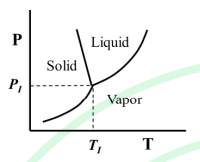
\includegraphics[width=0.5\columnwidth]{figs/fig12.png}
    \caption{}
    \label{fig:placeholder}
\end{figure}



\hfill[GATE XE 2025]

\begin{figure}[H]
    \centering
    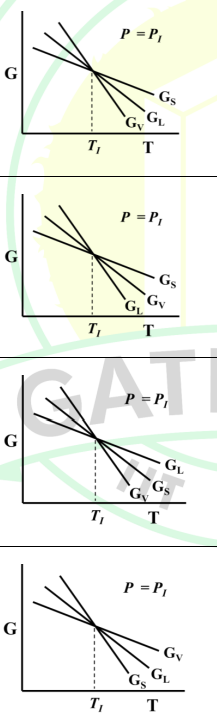
\includegraphics[width=0.3\columnwidth]{figs/fig13.png}
    \caption{}
    \label{fig:placeholder}
\end{figure}
\item The TTT diagram for eutectoid steel is shown below. The steel after complete austenitization at 1073 K is rapidly cooled to different temperatures and held for varying times (as indicated in Column I) followed by quenching to 300 K. Assuming isothermal transformation, match the heat treatment conditions in Column I with the corresponding microstructure in Column II.

\hfill[GATE XE 2025]

\begin{center}
\begin{tabular}{l l}
\textbf{Column I} & \textbf{Column II} \\
(P) Held at 300 K indefinitely & (1) Bainite \\
(Q) Held at 873 K for 4 minutes & (2) Martensite \\
(R) Held at 673 K for 20 minutes & (3) Pearlite \\
(S) Held at 623 K for 2 minutes & (4) Bainite + Martensite \\
\end{tabular}
\end{center}

\begin{figure}[H]
    \centering
    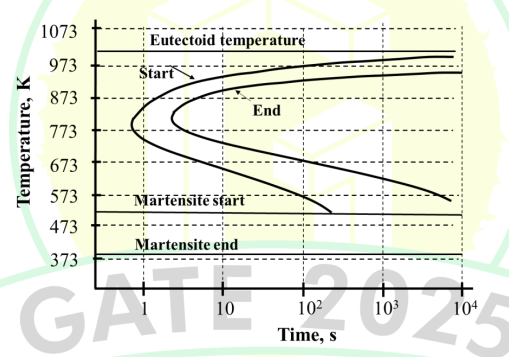
\includegraphics[width=0.5\columnwidth]{figs/fig14.png}
    \caption{}
    \label{fig:placeholder}
\end{figure}

\hfill[GATE XE 2025]

\begin{multicols}{2}
\begin{enumerate}
\item P -- 3; Q -- 2; R -- 1; S -- 4
\item P -- 2; Q -- 3; R -- 1; S -- 4
\item P -- 2; Q -- 1; R -- 3; S -- 4
\item P -- 4; Q -- 3; R -- 1; S -- 2
\end{enumerate}
\end{multicols}

\item A diffraction pattern is obtained from a powdered sample of a pure element, which has FCC crystal structure. If $x$ and $y$ are the Bragg angles of the first and the third peaks, respectively, then the ratio, $\dfrac{\sin y}{\sin x}$, is (rounded off to one decimal place) \rule{3cm}{0.15mm}

\hfill[GATE XE 2025]

\item For a pure element with a BCC crystal structure, the surface energies per unit area of $\{100\}$ and $\{110\}$ free surfaces are $S_{100}$ and $S_{110}$, respectively. The ratio, $\dfrac{S_{100}}{S_{110}}$, is (rounded off to one decimal place) \rule{3cm}{0.15mm}

\hfill[GATE XE 2025]

\item On applying $10~\mathrm{V}$ across the two ends of a $100~\mathrm{cm}$ long copper wire, the average drift velocity (in $\mathrm{cm\, s^{-1}}$) in the wire is (rounded off to two decimal places) \rule{3cm}{0.15mm} \\
\textit{Given:} Electron density of copper $= 8.43 \times 10^{22}~\mathrm{cm^{-3}}$; \\
Copper resistivity $= 1.67 \times 10^{-6}~\Omega\,\mathrm{cm}$; \\
Electron charge $= 1.6 \times 10^{-19}~\mathrm{C}$

\hfill[GATE XE 2025]

\item An aluminum transmission line of $7~\mathrm{km}$ length is designed to carry $100~\mathrm{A}$ current with no more than $2~\mathrm{MW}$ power loss. The required minimum diameter (in mm) of the transmission line is (rounded to the two decimal places) \rule{3cm}{0.15mm} \\
\textit{Given:} Aluminum conductivity $= 3.77 \times 10^{5}~\Omega^{-1}\,\mathrm{cm^{-1}}$

\hfill[GATE XE 2025]

\item An electric field is applied on a copper plate such that the electrons are displaced by $1.1 \times 10^{-18}~\mathrm{m}$ relative to the nucleus. The electronic polarization (in $\mu\mathrm{C\, m^{-2}}$) is (rounded off to two decimal places) \rule{3cm}{0.15mm} \\
\textit{Given:} Atomic number of copper $=29$; Copper has FCC crystal structure with lattice parameter $= 0.362~\mathrm{nm}$; Electron charge $= 1.6 \times 10^{-19}~\mathrm{C}$

\hfill[GATE XE 2025]

\item The standard free energy change for the reaction, $\mathrm{SO_2} + \dfrac{1}{2}{O_2} \rightleftharpoons \mathrm{SO_3}$ at equilibrium is given by $\Delta G^\circ = -94600 + 89.37\,T$, where $T$ is in Kelvin and $\Delta G^\circ$ is in Joule. The equilibrium constant $(K_P)$ at $1050~\mathrm{K}$ is (rounded off to two decimal places) \rule{3cm}{0.15mm} \\
\textit{Given:} Universal gas constant $(R) = 8.314~\mathrm{J\, K^{-1}\, mol^{-1}}$

\hfill[GATE XE 2025]

\item The slopes of reduction potential versus pH plots for the two reactions, ${NiO} + 2\mathrm{H}^+ + 2e^- \rightleftharpoons \mathrm{Ni} + \mathrm{H_2O}$ and $2\mathrm{H}^+ + 2e^- \rightleftharpoons \mathrm{H_2}$, at $298~\mathrm{K}$ and one atmospheric pressure are $S_1$ and $S_2$, respectively. The ratio $\dfrac{S_1}{S_2}$ is (rounded off to one decimal place) \rule{3cm}{0.15mm}

\hfill[GATE XE 2025]

\item At $873~\mathrm{K}$, hydrogen diffuses under steady state condition through a $5~\mathrm{mm}$ thick palladium sheet with a cross-sectional area of $0.3~\mathrm{m^2}$. The concentrations of hydrogen at high and low pressure ends of the sheet are $3~\mathrm{kg\, m^{-3}}$ and $0.5~\mathrm{kg\, m^{-3}}$, respectively. The amount of hydrogen (in kg per day) passing through the sheet is (rounded off to two decimal places) \rule{3cm}{0.15mm} \\
\textit{Given:} At $873~\mathrm{K}$, diffusivity of hydrogen $= 1.8 \times 10^{-8}~\mathrm{m^2\, s^{-1}}$

\hfill[GATE XE 2025]

\item Corrosion of pure iron takes place in an acidic electrolyte by forming $\mathrm{Fe^{2+}}$ ions at ambient condition. The corrosion current density is measured to be $2 \times 10^{-4}~\mathrm{A\, cm^{-2}}$. The corrosion rate (in mm per year) of iron is (rounded off to one decimal place) \rule{3cm}{0.15mm} \\
\textit{Given:} Atomic weight of iron $= 55.85$; Density of iron $= 7.86~\mathrm{g\, cm^{-3}}$; Consider 365 days in a year; $1$ Faraday $= 96500~\mathrm{C\, mol^{-1}}$

\hfill[GATE XE 2025]

\item Consider a spring-mass system with mass $m$ and spring stiffness $k$ as shown in the illustration. At time $t=0$, the mass is displaced by $P$ units and the velocity of the mass is zero. The displacement of the mass, $x(t)$, is measured from the equilibrium position.

Which one of the following functions represent $x(t)$?
% :contentReference[oaicite:0]{index=0}

\begin{figure}[H]
    \centering
    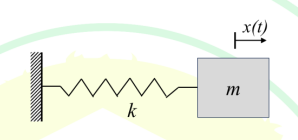
\includegraphics[width=0.5\columnwidth]{figs/fig15.png}
    \caption{}
    \label{fig:placeholder}
\end{figure}

\hfill[GATE XE 2025]


\begin{multicols}{2}
\begin{enumerate}
\item $P\sin\!\big(\sqrt{k/m}\,t\big)$
\item $\dfrac{P}{2}\cos\!\big(\sqrt{k/m}\,t\big)+\dfrac{P}{2}\sin\!\big(\sqrt{k/m}\,t\big)$
\item $P\cos\!\big(\sqrt{k/m}\,t\big)$
\item $P\cos\!\big(\sqrt{k/m}\,t\big)+P\sin\!\big(\sqrt{k/m}\,t\big)$
\end{enumerate}
\end{multicols}

\item A ball of mass $5m$ approaches a stationary ball of mass $m$ with a horizontal velocity of $2~\text{m/s}$ from left to right. After a perfectly elastic central collision, the horizontal velocity of the heavier ball is $1~\text{m/s}$ from left to right.

Which one of the following statements, regarding the velocity (in m/s) of the lighter ball after impact, is TRUE?
% :contentReference[oaicite:1]{index=1}


\hfill[GATE XE 2025]


\begin{multicols}{2}
\begin{enumerate}
\item Comes to rest
\item Moves from left to right at $5~\text{m/s}$
\item Moves from right to left at $5~\text{m/s}$
\item Moves from left to right at $1~\text{m/s}$
\end{enumerate}
\end{multicols}

\item The Mohr’s circle corresponding to an infinitesimal element is shown in the figure. The plane $PQ$ in the infinitesimal element, at an angle of $\theta$ from the $x$-axis, is in a state of pure shear.

Which one of the following values of $\theta$ (in degrees) is CORRECT?
% :contentReference[oaicite:2]{index=2}
\begin{figure}[H]
    \centering
    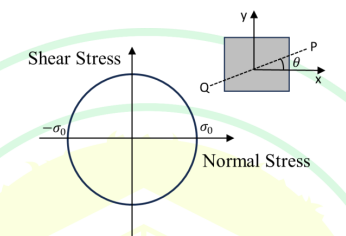
\includegraphics[width=0.5\columnwidth]{figs/fig16.png}
    \caption{}
    \label{fig:placeholder}
\end{figure}

\hfill[GATE XE 2025]


\begin{multicols}{2}
\begin{enumerate}
\item 90
\item 60
\item 45
\item 120
\end{enumerate}
\end{multicols}

\item The two-dimensional state of stress, in an infinitesimal element, is given by $\sigma_{xx}=800~\text{MPa}$, $\sigma_{xy}=300~\text{MPa}$ and $\sigma_{yy}=0~\text{MPa}$.

Which one of the following options is the maximum shear stress (in MPa) in the element?
% :contentReference[oaicite:3]{index=3}


\hfill[GATE XE 2025]


\begin{multicols}{2}
\begin{enumerate}
\item 500
\item 400
\item 800
\item 300
\end{enumerate}
\end{multicols}

\item Two cars $P$ and $Q$ are travelling on a straight path and are $60~\text{m}$ apart as shown in the figure; Car $P$ is moving with a constant velocity of $36~\text{kmph}$, while car $Q$ is moving at a constant velocity of $18~\text{kmph}$. At this instant, the driver in car $P$ applies the brake and collision occurs with car $Q$ after $30$ seconds.

Assuming uniform deceleration due to braking, which one of the following is the CORRECT velocity (in m/s) of the car $P$ just before the collision?
% :contentReference[oaicite:4]{index=4}
\begin{figure}[H]
    \centering
    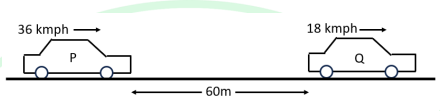
\includegraphics[width=0.5\columnwidth]{figs/fig17.png}
    \caption{}
    \label{fig:placeholder}
\end{figure}

\hfill[GATE XE 2025]


\begin{multicols}{2}
\begin{enumerate}
\item 1
\item 16
\item 5
\item 4
\end{enumerate}
\end{multicols}

\item The natural frequency of a spring-mass system is $10~\text{rad/s}$.

Which of the following statements is/are CORRECT?
% (Options for Q.71 are on the same page as Q.70)
% :contentReference[oaicite:5]{index=5}


\hfill[GATE XE 2025]


\begin{multicols}{2}
\begin{enumerate}
\item The mass is $100~\text{kg}$ and the stiffness is $1~\text{N/m}$.
\item The mass is $1.25~\text{kg}$ and the stiffness is $125~\text{N/m}$.
\item The stiffness is $620~\text{N/m}$ and the mass is $6.2~\text{kg}$.
\item The stiffness is $62~\text{N/m}$ and the mass is $620~\text{kg}$.
\end{enumerate}
\end{multicols}

\item Consider a beam with a square box cross-section as shown in the figure. The outer square has a length of $10~\text{mm}$. The thickness of the section is $1~\text{mm}$.

The area moment of inertia about the $x$-axis is \rule{3cm}{0.15mm} $\text{mm}^4$ (in integer).
% :contentReference[oaicite:6]{index=6}
\begin{figure}[H]
    \centering
    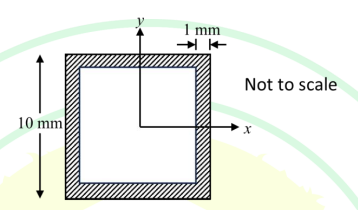
\includegraphics[width=0.5\columnwidth]{figs/fig18.png}
    \caption{}
    \label{fig:placeholder}
\end{figure}

\hfill[GATE XE 2025]


\item For a certain linear elastic isotropic material, the Young’s modulus is $140~\text{GPa}$ and the shear modulus is $50~\text{GPa}$.

The Poisson’s ratio for the material is \rule{3cm}{0.15mm} (rounded off up to two decimal places).
% :contentReference[oaicite:7]{index=7}


\hfill[GATE XE 2025]


\item A force of $P=100~\text{N}$ is applied at the ends of the pliers as shown in the figure.

Neglecting friction, the force exerted by the upper jaw on the workpiece is \rule{3cm}{0.15mm} N (in integer).
% :contentReference[oaicite:8]{index=8}
\begin{figure}[H]
    \centering
    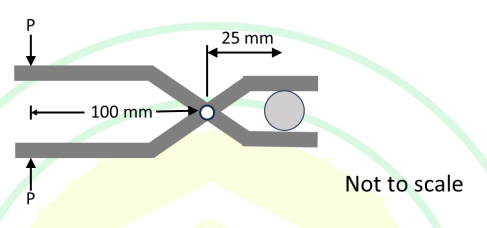
\includegraphics[width=0.5\columnwidth]{figs/fig19.png}
    \caption{}
    \label{fig:placeholder}
\end{figure}

\hfill[GATE XE 2025]


\item Consider two blocks, $P$ of mass $100~\text{kg}$ and $Q$ of mass $150~\text{kg}$, resting as shown in the figure. The angle $\theta=30^\circ$. The coefficient of friction between the two blocks is $0.2$. Assume no friction exists at all other interfaces. The minimum force required to move the block $P$ upward is $W$.

Which one of the following options is closest to the CORRECT magnitude of $W$ (in N)?
% :contentReference[oaicite:9]{index=9}
\begin{figure}[H]
    \centering
    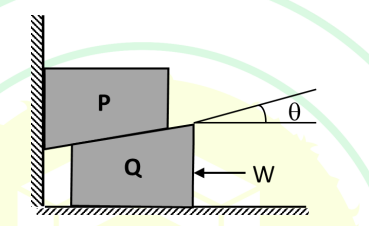
\includegraphics[width=0.5\columnwidth]{figs/fig20.png}
    \caption{}
    \label{fig:placeholder}
\end{figure}

\hfill[GATE XE 2025]


\begin{multicols}{2}
\begin{enumerate}
\item 862.2
\item 1116.6
\item 2900.0
\item 406.2
\end{enumerate}
\end{multicols}

\item Which one of the following vertical columns, of circular cross-section, sustains the highest load without buckling?
% :contentReference[oaicite:10]{index=10}


\hfill[GATE XE 2025]


\begin{multicols}{2}
\begin{enumerate}
\item Cantilever column with a length $L$ and cross-section diameter $d$
\item Column with hinge at one end and roller at the other end with a length $2L$ and cross-section diameter $d$
\item Cantilever column with a length $L$ and cross-section diameter $2d$
\item Column with hinge at one end and roller at the other end with a length $L$ and cross-section diameter $d$
\end{enumerate}
\end{multicols}

\item The figure shows a rod $PQ$, hinged at $P$, rotating counter-clockwise with a uniform angular speed of $15~\text{rad/s}$. A block $R$ translates along a slot cut out in rod $PQ$. At the instant shown the distance $PR=0.5~\text{m}$ and $\theta=60^\circ$. The relative velocity of $R$ with respect to the rod $PQ$ is $5~\text{m/s}$ at the instant shown. The relative acceleration of $R$ with respect to the rod $PQ$ is zero at the instant shown.

Which one of the following is the CORRECT magnitude of the absolute acceleration (in $\text{m/s}^2$) of block $R$?
% :contentReference[oaicite:11]{index=11}

\begin{figure}[H]
    \centering
    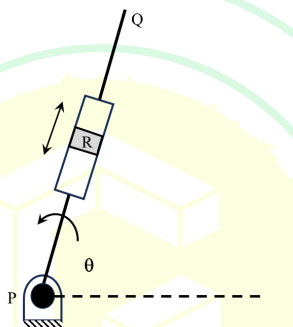
\includegraphics[width=0.5\columnwidth]{figs/fig21.png}
    \caption{}
    \label{fig:placeholder}
\end{figure}

\hfill[GATE XE 2025]


\begin{multicols}{2}
\begin{enumerate}
\item 135.2
\item 187.5
\item 112.5
\item 150.0
\end{enumerate}
\end{multicols}

\item The frame shown in the figure is loaded at $S$ with a force of $2000~\text{N}$. The reactions at $T$ are denoted by $T_x$ and $T_y$, while the reaction at $W$ is $W_y$. Neglect the weight of the members.

Which one of the following options for the magnitudes of the forces (in N), $T_x$, $T_y$ and $W_y$, is CORRECT?
% :contentReference[oaicite:12]{index=12}
\begin{figure}[H]
    \centering
    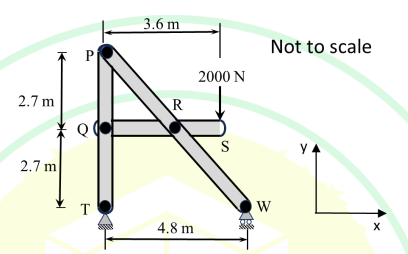
\includegraphics[width=0.5\columnwidth]{figs/fig22.png}
    \caption{}
    \label{fig:placeholder}
\end{figure}

\hfill[GATE XE 2025]


\begin{multicols}{2}
\begin{enumerate}
\item $T_x=0$, $T_y=1000$ and $W_y=1000$
\item $T_x=0$, $T_y=1500$ and $W_y=500$
\item $T_x=0$, $T_y=800$ and $W_y=1200$
\item $T_x=0$, $T_y=500$ and $W_y=1500$
\end{enumerate}
\end{multicols}

\item A closed thin cylindrical tank with a mean diameter $d=300~\text{mm}$ and thickness $t=2~\text{mm}$, is subjected to a uniform internal gas pressure $p$. The allowable shear stress on the curved wall of the tank is $70~\text{MPa}$.

Based on the Tresca criteria, which one of the following options for the maximum safe value of $p$ (in MPa) is CORRECT?
% :contentReference[oaicite:13]{index=13}


\hfill[GATE XE 2025]


\begin{multicols}{2}
\begin{enumerate}
\item 3.73
\item 7.46
\item 1.87
\item 5.60
\end{enumerate}
\end{multicols}

\item An infinitesimal square element $PQRS$ is shown in the figure. The $x$ and $y$ axes are also marked in the figure. The strains on the element are given by \\ $\varepsilon_{xx}=500\times10^{-6}$, $\varepsilon_{yy}=100\times10^{-6}$ and $\varepsilon_{xy}=0$.\\

Which of the following statements is/are CORRECT?
% :contentReference[oaicite:14]{index=14}
\begin{figure}[H]
    \centering
    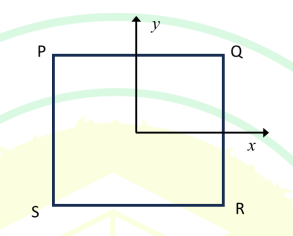
\includegraphics[width=0.5\columnwidth]{figs/fig23.png}
    \caption{}
    \label{fig:placeholder}
\end{figure}

\hfill[GATE XE 2025]


\begin{multicols}{2}
\begin{enumerate}
\item Percentage change in length of the diagonal $PR$ is $0.03$.
\item Change in angle between $PR$ and $QS$ is $4\times10^{-4}~\text{rad}$.
\item Change in angle between $PR$ and $QS$ is $2\times10^{-4}~\text{rad}$.
\item Percentage change in length of the diagonal $QS$ is $0.03$.
\end{enumerate}
\end{multicols}

\item The figure shows the stress distribution across an internal surface of a rectangular beam of height $30~\text{mm}$ and depth $10~\text{mm}$. The normal stress distribution is given by the expression $\sigma_{xx}=200y+500~\text{N/mm}^2$; $y$ is the distance in mm from the centroidal axis of the beam. Assume that there is no variation in the stress distribution along the $z$-direction.

Which of the following statements is/are CORRECT?
% :contentReference[oaicite:15]{index=15}
\begin{figure}[H]
    \centering
    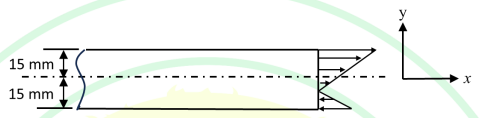
\includegraphics[width=0.5\columnwidth]{figs/fig24.png}
    \caption{}
    \label{fig:placeholder}
\end{figure}

\hfill[GATE XE 2025]


\begin{multicols}{2}
\begin{enumerate}
\item The net force in the $x$ direction is $150~\text{kN}$.
\item The net force in the $x$ direction is $75~\text{kN}$.
\item The net moment about the $z$ axis is $4500~\text{Nm}$.
\item The net moment about the $z$ axis is $2250~\text{Nm}$.
\end{enumerate}
\end{multicols}

\item A vertical column fixed at one end is subjected to a compressive axial load at the free end. The column’s section modulus, $EI$, is $9.82\times10^{5}~\text{Nm}^2$ and the cross-section area is $7.85\times10^{-3}~\text{m}^2$. The length of the column is $2~\text{m}$. The yield stress of the material is $145~\text{MPa}$.

If the column can fail either in buckling or by Tresca’s criterion, the maximum load that the structure can safely sustain is \rule{3cm}{0.15mm} kN (rounded off to one decimal place).
% :contentReference[oaicite:16]{index=16}


\hfill[GATE XE 2025]


\item A simply-supported beam, with a point load $P=150~\text{kN}$ at a distance of $L/3$ from the left end, is shown in the figure. The elastic-strain energy $(U)$ of the beam is given by the following expression:
\begin{align}
U=\frac{2}{243}\,\frac{P^{2}L^{3}}{EI}
\end{align}
where the section modulus, $EI$, is $16.66\times10^{5}~\text{Nm}^2$ and the length of the beam $L$ is $1~\text{m}$.

The deflection at the loading point is \rule{3cm}{0.15mm} mm (rounded off to two decimal places).
% :contentReference[oaicite:17]{index=17}
% (expression line from :contentReference[oaicite:18]{index=18})

\begin{figure}[H]
    \centering
    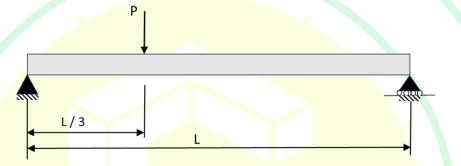
\includegraphics[width=0.5\columnwidth]{figs/fig25.png}
    \caption{}
    \label{fig:placeholder}
\end{figure}


\hfill[GATE XE 2025]


\item A simply-supported beam has a circular cross-section with a diameter of $20~\text{mm}$, area of $314.2~\text{mm}^2$, area moment of inertia of $7854~\text{mm}^4$ and a length $L$ of $4~\text{m}$. A point load $P=100~\text{N}$ acts at the center and an axial load $Q=20~\text{kN}$ acts through the centroidal axis as shown in the figure.

The magnitude of the offset between the neutral axis and the centroidal axis, at $L/2$ from the left, is \rule{3cm}{0.15mm} mm (rounded off to one decimal place).
% :contentReference[oaicite:19]{index=19}

\begin{figure}[H]
    \centering
    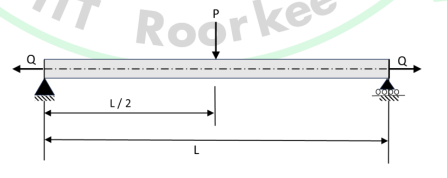
\includegraphics[width=0.5\columnwidth]{figs/fig26.png}
    \caption{}
    \label{fig:placeholder}
\end{figure}

\hfill[GATE XE 2025]


\item A massless cantilever beam, with a tip mass $m$ of $10~\text{kg}$, is modeled as an equivalent spring-mass system as shown in the figure. The beam is of length $L=1~\text{m}$, with a circular cross-section of diameter $d=20~\text{mm}$. The Young’s modulus of the beam material is $200~\text{GPa}$.

The natural frequency of the spring-mass system is \rule{3cm}{0.15mm} Hz (rounded off to two decimal places).
% :contentReference[oaicite:20]{index=20}

\begin{figure}[H]
    \centering
    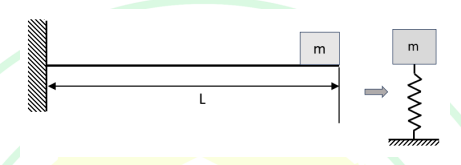
\includegraphics[width=0.5\columnwidth]{figs/fig27.png}
    \caption{}
    \label{fig:placeholder}
\end{figure}

\hfill[GATE XE 2025]


\item An electric motor’s rotor is spinning at $1500~\text{rpm}$ when its load and power are cut-off. The rotor which has a mass of $50~\text{kg}$ and a radius of gyration of $200~\text{mm}$, then coasts down to rest. Due to kinetic friction, a constant torque of $10~\text{Nm}$ acts on the rotor as it coasts down.

The number of revolutions executed by the rotor before it comes to rest is \rule{3cm}{0.15mm} (in integer).
% :contentReference[oaicite:21]{index=21}


\hfill[GATE XE 2025]


\item A bar of length $L=1~\text{m}$ is fixed at one end. Before heating its free end has a gap of $\delta=0.1~\text{mm}$ from a rigid wall as shown in the figure. Now the bar is heated resulting in a uniform temperature rise of $10~^\circ\text{C}$. The coefficient of linear thermal expansion of the material is $20\times10^{-6}/^\circ\text{C}$ and the Young’s modulus of elasticity is $100~\text{GPa}$. Assume that the material properties do not change with temperature.

The magnitude of the resulting axial stress on the bar is \rule{3cm}{0.15mm} MPa (in integer).
% :contentReference[oaicite:22]{index=22}
\begin{figure}[H]
    \centering
    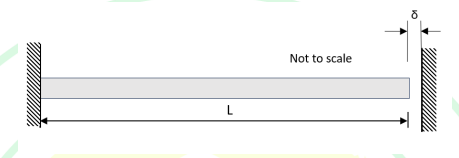
\includegraphics[width=0.5\columnwidth]{figs/fig28.png}
    \caption{}
    \label{fig:placeholder}
\end{figure}

\hfill[GATE XE 2025]

\item  A tank is divided into two compartments with one compartment containing a gas at a given pressure, while the second is completely evacuated. If the partition is removed, the gas occupies the entire compartment. Which one of the following statements is CORRECT?

\hfill[GATE XE 2025]
\begin{multicols}{2}
\begin{enumerate}
\item Work done is equal to the area under the curve of a $p\!-\!V$ diagram
\item Expansion of gas is not restrained by external force
\item The entire process is reversible
\item The overall change in volume is zero for the entire system
\end{enumerate}
\end{multicols}

\item A cylinder of volume 0.1 m$^3$ is filled with nitrogen at 10 MPa and 300 K. Consider nitrogen to be an ideal gas. The cylinder develops a leak and nitrogen escapes to atmosphere which is at 0.1 MPa. After sometime, the pressure in the cylinder reduces to 5 MPa. Assuming the cylinder and the leaked gas temperature remains constant at 300 K, the work done (in MJ) by nitrogen gas is
\hfill[GATE XE 2025]
\begin{multicols}{2}
\begin{enumerate}
\item 0.1
\item 1
\item 0.5
\item 10
\end{enumerate}
\end{multicols}

\item A closed system undergoes a process 1–2 in which it absorbs 150 kJ of energy as heat and does 90 kJ of work. Then it follows another process 2–3 in which 80 kJ of work is done on it while it rejects 60 kJ as heat. If it is desired to restore the system to the initial state (state 1) by an adiabatic path, the work interaction (in kJ) in this process will be
\hfill[GATE XE 2025]
\begin{multicols}{2}
\begin{enumerate}
\item 80
\item 100
\item 50
\item 70
\end{enumerate}
\end{multicols}

\item The inlet and outlet temperatures of the flowing fluid during a steady state flow process are the same as that of the surroundings. If the changes in kinetic and potential energies are neglected, the maximum power that can be obtained is equal to
\hfill[GATE XE 2025]
\begin{multicols}{2}
\begin{enumerate}
\item the rate of increase in enthalpy of the flowing fluid
\item the rate of decrease in Helmholtz energy of the flowing fluid
\item the rate of decrease in Gibbs free energy of the flowing fluid
\item the rate of decrease in internal energy of the flowing fluid
\end{enumerate}
\end{multicols}

\item If $\gamma$ refers to the ratio of specific heats, the air-standard efficiency of an Otto cycle is
\hfill[GATE XE 2025]
\begin{multicols}{2}
\begin{enumerate}
\item $1-\dfrac{1}{(\text{Compression ratio})^{\gamma}}$
\item $1-\dfrac{1}{(\text{Pressure ratio})^{\brak{\frac{\gamma-1}{\gamma}}}}$
\item $1-\dfrac{1}{(\text{Compression ratio})^{(\gamma-1)}}$
\item $1-\dfrac{1}{(\text{Pressure ratio})^{(\gamma-1)}}$
\end{enumerate}
\end{multicols}

\item Let $T_H$ and $T_L$ denote the absolute temperatures of high and low temperature reservoirs, respectively. The coefficient of performance of a reversible refrigerator operating between these two reservoirs is
\hfill[GATE XE 2025]
\begin{multicols}{2}
\begin{enumerate}
\item $\dfrac{1}{\dfrac{T_H}{T_L}-1}$
\item $\dfrac{1}{1-\dfrac{T_H}{T_L}}$
\item $\dfrac{1}{\dfrac{T_L}{T_H}-1}$
\item $\dfrac{1}{\dfrac{T_L}{T_H}+1}$
\end{enumerate}
\end{multicols}

\item A tank of 4 m$^3$ contains an ideal gas mixture of 60\% hydrogen and 40\% nitrogen by volume at 100 kPa and 300 K. Nitrogen is added to the tank such that the composition changes to 50\% nitrogen by volume, with a final temperature of 300 K. The amount of nitrogen (in kmol) to be added is \rule{3cm}{0.15mm} (rounded off to three decimal places). Use: Universal gas constant $(R_u)=8.314\ \mathrm{kJ/(kmol\!-\!K)}$.
\hfill[GATE XE 2025]

\item A heat engine having thermal efficiency of 40\% receives heat from a source at 600 K and rejects heat to a sink at 300 K. The second-law efficiency (in \%) of this engine is \rule{3cm}{0.15mm} (answer in integer).
\hfill[GATE XE 2025]

\item A rigid tank of 300 litre capacity contains 3 kg of oxygen (molar mass $=32\ \mathrm{kg/kmol}$) at 25 $^\circ$C. If oxygen behaves as an ideal gas, the pressure (in kPa) inside the tank is \rule{3cm}{0.15mm} (rounded off to two decimal places). Use: Universal gas constant $(R_u)=8.314\ \mathrm{kJ/(kmol\!-\!K)}$.
\hfill[GATE XE 2025]

\item For an ideal gas turbine cycle, $T_1$ and $T_3$ are the compressor inlet temperature and turbine inlet temperature respectively. The ratio $\dfrac{T_3}{T_1}$ is denoted by $t$ and the ratio of specific heats is denoted by $\gamma$. For any given $t$, the optimum pressure ratio for the maximum specific work output is
\hfill[GATE XE 2025]
\begin{multicols}{2}
\begin{enumerate}
\item $\dfrac{t^{\frac{1}{2(\gamma-1)}}}{}$
\item $\dfrac{t^{\frac{\gamma}{2(\gamma-1)}}}{}$
\item $t^{\frac{\gamma}{(\gamma-1)}}$
\item $t^{\frac{1}{\gamma-1}}$
\end{enumerate}
\end{multicols}

\item For a pure substance that expands on freezing, which of the following statement(s) is/are CORRECT?
\hfill[GATE XE 2025]
\begin{multicols}{2}
\begin{enumerate}
\item Temperature of the liquid phase can be lower than the temperature at the triple point
\item Critical pressure is equal to the pressure at the triple point
\item Highest pressure at which the vapour phase can exist is the pressure at the triple point
\item Highest temperature at which solid–liquid phase change can happen is the temperature at the triple point
\end{enumerate}
\end{multicols}

\item Consider a gas obeying the relation $(P)(v-b)=RT$, where $b$ and $R$ are constants. Which of the following statement(s) is/are CORRECT about the specific heat capacity at constant pressure?
\hfill[GATE XE 2025]
\begin{multicols}{2}
\begin{enumerate}
\item It is independent of temperature
\item It is a function of pressure
\item It is a function of temperature
\item It is independent of both specific volume and pressure
\end{enumerate}
\end{multicols}

\item A piston–cylinder arrangement contains an ideal gas mixture of 4 kg of hydrogen and 13 kg of nitrogen at 250 K and atmospheric pressure. On heat addition, the mixture expands at constant pressure until the temperature rises to 350 K. The change in entropy (in kJ/K) of the mixture is \rule{3cm}{0.15mm} (rounded off to three decimal places). Take the constant-pressure specific heats as: Hydrogen $c_{p,H_2}=14.43\ \mathrm{kJ/(kmol\!-\!K)}$; Nitrogen $c_{p,N_2}=29.10\ \mathrm{kJ/(kmol\!-\!K)}$; Universal gas constant $R_u=8.314\ \mathrm{kJ/(kmol\!-\!K)}$.

\hfill[GATE XE 2025]

\item Air in an ideal Diesel cycle is compressed from 3 litre to 0.15 litre. It then expands during a constant pressure heat addition process to 0.3 litre. If the ratio of specific heats, $\gamma=1.4$, the thermal efficiency (in \%) of the cycle is \rule{3cm}{0.15mm} (rounded to one decimal place).

\item Air at 101 kPa, 15 $^\circ$C and 50\% relative humidity is first heated to 20 $^\circ$C in a heating coil, and then humidified by spraying water on it. In the final state, the air has temperature of 25 $^\circ$C and relative humidity of 85\%. The amount of water sprayed (in gm per kg of dry air) is \rule{3cm}{0.15mm}(rounded off to two decimal places).
Use the following data:
The saturation pressure of water at 15 $^\circ$C = 1.7057 kPa
The saturation pressure of water at 25 $^\circ$C = 3.1698 kPa.

\item Superheated steam at 2 MPa, 350 $^\circ$C is mixed adiabatically with superheated steam at 2 MPa, 400 $^\circ$C. The mass flow rates of the streams are 3 kg/min and 2 kg/min, respectively. This mixture then expands in an adiabatic nozzle to a saturated mixture with quality of 0.77 and 1 kPa. Neglect the velocity at the nozzle entrance and the change in potential energies. The velocity at the nozzle exit (in m/s) is \rule{3cm}{0.15mm} (rounded off to two decimal places). Use: At 2 MPa, 300 $^\circ$C: $h=3024.2$ kJ/kg; At 2 MPa, 400 $^\circ$C: $h=3248.4$ kJ/kg; At 1 kPa: $h_f=29.3$ kJ/kg, $h_g=2513.7$ kJ/kg.
\hfill[GATE XE 2025]

\item A piston–cylinder assembly having 250 mm diameter contains 0.01 kg of water vapor at 1 MPa and 200 $^\circ$C. The specific volume of the vapor is $0.20602\ \mathrm{m^3/kg}$. The system expands as per the relation $pV^n=\text{constant}$, where $p$ is pressure and $V$ is volume. The expansion of water vapour displaces the piston by 50 mm. If the final pressure is 0.35 MPa, the value of the exponent $(n)$ is \rule{3cm}{0.15mm} (rounded off to two decimal places).
\hfill[GATE XE 2025]

\item Air enters a hair dryer at 22 $^\circ$C and 100 kPa with a velocity of 3.7 m/s, and leaves the dryer at 83 $^\circ$C and 100 kPa with a velocity of 9.1 m/s. The exit area of the dryer is 18.7 cm$^2$, and the ambient temperature is 22 $^\circ$C. The air is an ideal gas with gas constant $R=0.287\ \mathrm{kJ/(kg\!-\!K)}$ and isobaric specific heat $c_p=1.005\ \mathrm{kJ/(kg\!-\!K)}$. If the change in potential energy is neglected, the second-law efficiency (in \%) of the dryer is \rule{3cm}{0.15mm} (rounded off to one decimal place).
\hfill[GATE XE 2025]

\item A steam boiler contains saturated water vapour at 200 $^\circ$C. After a certain period, the temperature of the boiler drops to 110 $^\circ$C. Assume that all the valves of the boiler are closed and the energy is lost as heat to the surroundings. The ratio of mass of liquid to the mass of vapour is \rule{3cm}{0.15mm} (rounded off to two decimal places). Saturated volume of vapour phase at 200 $^\circ$C $=0.127\ \mathrm{m^3/kg}$; at 110 $^\circ$C $=1.210\ \mathrm{m^3/kg}$; saturated volume of liquid phase at 110 $^\circ$C $=0.001\ \mathrm{m^3/kg}$.
\hfill[GATE XE 2025]

\item Two Carnot heat engines (E$_1$ and E$_2$) are operating in series. Engine E$_1$ receives heat from a reservoir at $T_H=1600\ \mathrm{K}$ and does work $W_1$. Engine E$_2$ receives heat from an intermediate reservoir at $T$, does work $W_2$ and rejects the rest to a reservoir at $T_L=400\ \mathrm{K}$. Both the engines have identical thermal efficiencies. The temperature $T$ (in K) of the intermediate reservoir is \rule{3cm}{0.15mm} (answer in integer).

\begin{figure}[H]
    \centering
    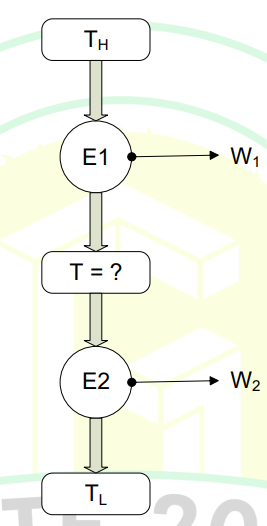
\includegraphics[width=0.3\columnwidth]{figs/fig29.png}
    \caption{}
    \label{fig:placeholder}
\end{figure}

\hfill[GATE XE 2025]

\item A particular temperature scale is obtained according to the relation: $t=a e^{b\alpha}$ where $a$ and $b$ are constants, and $t$ is in $^\circ$C. The thermometric property as measured by the thermometer is $\alpha$. The values of $\alpha$ at ice point and steam point are 6 and 9, respectively. The temperature (in $^\circ$C) which gives $\alpha=7$ is \rule{3cm}{0.15mm} (rounded off to two decimal places).
\hfill[GATE XE 2025]

\item In a piston cylinder assembly, one kmol of an ideal gas is compressed from an initial state of 200 kPa and 400 K to a final state of 1 MPa and 400 K. If the surroundings are at 400 K, the minimum amount of work (in kJ/kmol) required for the compression process is \rule{3cm}{0.15mm} (rounded off to two decimal places). Use: Universal gas constant $(R_u)=8.314\ \mathrm{kJ/(kmol\!-\!K)}$.
\hfill[GATE XE 2025]

\item Which one of the following measures of viscosity is dimensionless?

\hfill[GATE XE 2025]

\begin{multicols}{2}
\begin{enumerate}
\item Inherent viscosity
\item Reduced viscosity
\item Zero-shear viscosity
\item Specific viscosity
\end{enumerate}
\end{multicols}

\item Which one of the following permits the direct determination of intrinsic viscosity of a polymer solution for known molecular weight of the polymer?

\hfill[GATE XE 2025]

\begin{multicols}{2}
\begin{enumerate}
\item Flory-Huggins equation
\item Newton’s law of viscosity
\item Williams-Landel-Ferry equation
\item Mark-Houwink equation
\end{enumerate}
\end{multicols}

\item Under which combination of conditions does the glass transition of a polymer increase?

\hfill[GATE XE 2025]

\begin{multicols}{2}
\begin{enumerate}
\item Increase in molecular weight and increase in plasticizer content
\item Increase in plasticizer content and decrease in cross-linking
\item Increase in branching and decrease in inter-chain interactions
\item Increase in chain length and decrease in plasticizer content
\end{enumerate}
\end{multicols}

\item In a polymer recycling plant, polymer ``X’’ was depolymerized by glycolysis in the presence of ethylene glycol and a suitable catalyst. The glycolysis reaction yielded the following compound:
\begin{figure}[H]
    \centering
    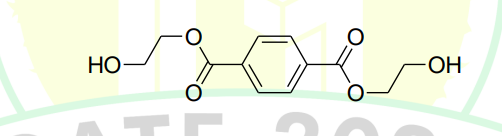
\includegraphics[width=0.5\columnwidth]{figs/fig30.png}
    \caption{}
    \label{fig:placeholder}
\end{figure}
Identify the polymer ``X’’ from the following options.

\hfill[GATE XE 2025]

\begin{multicols}{2}
\begin{enumerate}
\item Poly(ethylene terephthalate)
\item Polystyrene
\item Acrylonitrile butadiene styrene
\item Poly(vinyl chloride)
\end{enumerate}
\end{multicols}

\item Polymer ``Z’’ has a high melting point and it decomposes even before it melts. Hence, it is usually dissolved and subsequently regenerated. Rayon is one such regenerated form. Identify the polymer ``Z’’ from the following options.

\hfill[GATE XE 2025]

\begin{multicols}{2}
\begin{enumerate}
\item Urea formaldehyde
\item Poly(vinyl carbazole)
\item Cellulose
\item Poly(vinyl acetate)
\end{enumerate}
\end{multicols}

\item Match the \textbf{Product} with the most appropriate \textbf{Processing Technique} employed.

\hfill[GATE XE 2025]

\begin{center}
\begin{tabular}{l l}
\textbf{Product} & \textbf{Processing Technique} \\
P. Rainboots & 3. Rotational molding \\
Q. Disposable plastic cups & 4. Thermoforming \\
R. Soft drink bottles & 1. Blow molding \\
S. Flexible films & 2. Calendering \\
\end{tabular}
\end{center}

\begin{multicols}{2}
\begin{enumerate}
\item P-3; Q-1; R-2; S-4
\item P-3; Q-4; R-1; S-2
\item P-1; Q-2; R-4; S-3
\item P-1; Q-3; R-4; S-2
\end{enumerate}
\end{multicols}

\item Crystallization is favored in polymer melts when the chain entanglement is \rule{3cm}{0.15mm} and only polymers with \rule{3cm}{0.15mm} molecular arrangement can crystallize.

\hfill[GATE XE 2025]

\begin{multicols}{2}
\begin{enumerate}
\item maximum, ordered
\item minimum, random
\item maximum, random
\item minimum, ordered
\end{enumerate}
\end{multicols}

\item Match the \textbf{Polymer} with the most suitable \textbf{Monomer combinations} from which it is synthesized.

\hfill[GATE XE 2025]

\begin{center}
\begin{tabular}{l l}
\textbf{Polymer} & \textbf{Monomer combinations} \\
P. Polyurethane & 4. Hexamethylene diisocyanate and tetramethylene glycol \\
Q. Epoxy & 3. Epichlorohydrin and bisphenol A \\
R. Polyimide & 2. Pyromellitic anhydride and p,p$^\prime$-diamino diphenyl ether \\
S. Polyester & 1. Maleic acid and propylene glycol \\
\end{tabular}
\end{center}

\begin{multicols}{2}
\begin{enumerate}
\item P-4; Q-3; R-2; S-1
\item P-4; Q-2; R-3; S-1
\item P-2; Q-1; R-4; S-3
\item P-2; Q-3; R-1; S-4
\end{enumerate}
\end{multicols}

\item Thermoplastic Polyurethane and Polyamide 6 both contain amide linkages, but when compared to Polyurethane, Polyamide 6 shows higher melting point due to \rule{3cm}{0.15mm}.

\hfill[GATE XE 2025]

\begin{multicols}{2}
\begin{enumerate}
\item Higher molecular rigidity
\item Higher degree of branching
\item Lower molecular rigidity
\item Lower degree of crosslinking
\end{enumerate}
\end{multicols}

\item Injection molding is typically used to make plastic parts. If the pressure at the gate is monitored as a function of time during the injection of a thermoplastic polymer, identify the profile that best describes this event. (Profiles P, Q, R, S are given.)

\begin{figure}[H]
    \centering
    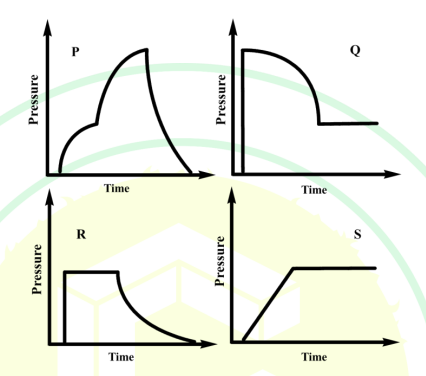
\includegraphics[width=0.5\columnwidth]{figs/fig31.png}
    \caption{}
    \label{fig:placeholder}
\end{figure}

\hfill[GATE XE 2025]

\begin{multicols}{2}
\begin{enumerate}
\item Q
\item R
\item P
\item S
\end{enumerate}
\end{multicols}

\item The `unperturbed dimension' of the polymer chain is represented as,
\begin{align}
    (\overline{r_0^2})^{1/2} \propto \bar{l}\,\bar{n}^{1/2}
\end{align}
where $(\overline{r_0^2})^{1/2}$ is the root-mean-square end-to-end distance, $\bar{l}$ is the average length of a segment and $n$ is the number of segments in the chain. Using the above, the root-mean-square end-to-end distance of a branched polyethylene would be \rule{3cm}{0.15mm} when compared with that of the linear polyethylene of the same molecular weight and the same number of segments.

\hfill[GATE XE 2025]

\begin{multicols}{2}
\begin{enumerate}
\item Same
\item Higher
\item Lower
\item Exactly $\sqrt{2}$ times
\end{enumerate}
\end{multicols}

\item Choose the option(s) that correctly match(es) the \textbf{Zones} with their typical \textbf{Functions} in an industrial extruder. (Tables/figure for Zones P, Q, R, S and Functions 1, 2, 3 are given.)\\
\begin{tabular}{|l|l|l|l|}
\hline
\multicolumn{2}{|c|}{\textbf{Zones}} & \multicolumn{2}{|c|}{\textbf{Functions}} \\
\hline
P & Feed zone & 1 & The melt acquires a constant flow rate \\
\hline
Q & Compression zone & 2 & No heating takes place \\
\hline
R & Metering zone & 3 & Polymer melts due to heat transferred from the heating element \\
\hline
& & 4 & The helical flight of the screw imparts constant flow of the melt \\
\hline
& & 5 & Polymer melts due to shear forces imparted by the screw \\
\hline
\end{tabular}

\hfill[GATE XE 2025]

\begin{multicols}{2}
\begin{enumerate}
\item P–3; Q–1; R–4; S–2
\item P–2; Q–4; R–3; S–1
\item P–4; Q–1; R–2; S–3
\item P–1; Q–3; R–2; S–4
\end{enumerate}
\end{multicols}



\item During material testing, stress is applied from time $t_i$ to $t_f$ as shown below.\\

\begin{figure}[H]
    \centering
    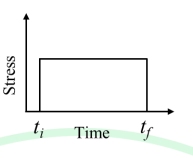
\includegraphics[width=0.3\columnwidth]{figs/fig32.png}
    \caption{}
    \label{fig:placeholder}
\end{figure}
The corresponding strain responses for three different materials are shown in plots P, Q and R.\\
\begin{figure}[H]
    \centering
    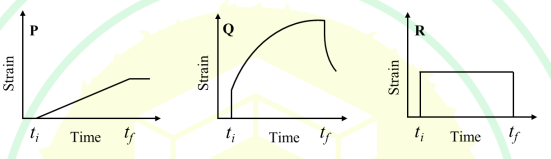
\includegraphics[width=0.5\columnwidth]{figs/fig33.png}
    \caption{}
    \label{fig:placeholder}
\end{figure}
Choose the option(s) where the strain response is correctly mapped to its material class.

\hfill[GATE XE 2025]

\begin{multicols}{2}
\begin{enumerate}
\item P- purely elastic; Q- purely viscous; R- viscoelastic
\item P- purely elastic; Q- viscoelastic; R- purely viscous
\item P- purely viscous; Q- purely elastic; R- viscoelastic
\item P- purely viscous; Q- viscoelastic; R- purely elastic
\end{enumerate}
\end{multicols}

\item Which option(s) correctly match(es) the \emph{Polymer property} with its appropriate \emph{Units}?

\begin{center}
\begin{tabular}{ll ll}
\multicolumn{2}{l}{\textbf{Polymer property}} & \multicolumn{2}{l}{\textbf{Units}}\\
P & Hildebrand solubility parameter & 1 & Pa\\
Q & Loss modulus & 2 & J m$^{-3}$\\
R & Toughness & 3 & (MPa)$^{1/2}$\\
S & Flexural strength & 4 & Kg m$^{-1}$ s$^{-2}$\\
\end{tabular}
\end{center}

\hfill[GATE XE 2025]

\begin{multicols}{2}
\begin{enumerate}
\item P-2; Q-1; R-3; S-4
\item P-2; Q-4; R-3; S-1
\item P-3; Q-1; R-2; S-4
\item P-3; Q-4; R-2; S-1
\end{enumerate}
\end{multicols}

\item Which option(s) correctly match(es) the \emph{Class of additives} used during polymer compounding with the corresponding \emph{Chemicals}?

\begin{center}
\begin{tabular}{ll ll}
\multicolumn{2}{l}{\textbf{Class of additives}} & \multicolumn{2}{l}{\textbf{Chemicals}}\\
P & Antioxidant     & 1 & Phthalocyanine\\
Q & Flame retardant & 2 & Di(2-ethylhexyl) phthalate\\
R & Plasticizer     & 3 & Tricresyl phosphate\\
S & Colorant        & 4 & Phenyl $\beta$-napthyl amine\\
\end{tabular}
\end{center}

\hfill[GATE XE 2025]

\begin{multicols}{2}
\begin{enumerate}
\item P-4; Q-3; R-2; S-1
\item P-4; Q-3; R-3; S-1
\item P-1; Q-2; R-4; S-2
\item P-2; Q-3; R-1; S-2
\end{enumerate}
\end{multicols}

\item In a set of copolymerization reactions, the following monomer reactivity ratios $(r_1$ and $r_2)$ were found for different cases.

\begin{center}
\begin{tabular}{c c c}
\textbf{Case} & $r_1$ & $r_2$\\
I   & 0.1   & 10\\
II  & 0.003 & 0.02\\
III & 3.4   & 5.6\\
IV  & 51    & 0.01\\
\end{tabular}
\end{center}

Which option(s) correctly identify/identifies the type of copolymerization corresponding to each Case?

\hfill[GATE XE 2025]

\begin{multicols}{2}
\begin{enumerate}
\item I — Ideal copolymerization
\item II — Azeotropic copolymerization
\item III — Block copolymerization
\item IV — Alternating copolymerization
\end{enumerate}
\end{multicols}

\item The crystallization of a polymer can only proceed in a temperature range limited to glass transition temperature ($T_g$) on the lower side, and the equilibrium melting point ($T_m^{\circ}$) on the higher side. Around $T_g$, the mobility of the polymer chains is lower, while in the proximity of $T_m^{\circ}$, crystal nucleation is inhibited. In a miscible polymer blend with only one component being crystalline, which option(s) correctly match(es) the \emph{Temperature conditions} with \emph{Events}?

\begin{center}
\begin{tabular}{ll ll}
\multicolumn{2}{l}{\textbf{Temperature conditions}} & \multicolumn{2}{l}{\textbf{Events}}\\
P & $T_g$ of the amorphous component is lower than the crystallizable one & 1 & Temperature range over which crystallization can occur becomes smaller\\
Q & $T_g$ of the amorphous component is higher than the crystallizable one & 2 & Crystallization is inhibited\\
R & Blend $T_g$ is higher than $T_m^{\circ}$ of the crystallizable one & 3 & Crystallization envelope $(T_m^{\circ}-T_g)$ is widened\\
  & & 4 & Crystallization is favored\\
\end{tabular}
\end{center}

\hfill[GATE XE 2025]

\begin{multicols}{2}
\begin{enumerate}
\item P-3; Q-2; R-4
\item P-3; Q-1; R-2
\item P-4; Q-1; R-3
\item P-4; Q-1; R-2
\end{enumerate}
\end{multicols}

\item The heat of polymerization of ethylene is 25 Kcal/mol. The amount of heat generated during the polymerization of 5.6 Kg polyethylene is \rule{3cm}{0.15mm} Kcal. (Round off to the nearest integer)

\hfill[GATE XE 2025]

\item The density of an amorphous polymer is 0.77 g cm$^{-3}$ and that of its crystalline counterpart is 0.99 g cm$^{-3}$. The density of a semi-crystalline sample of this polymer is found to be 0.88 g cm$^{-3}$. The degree of crystallinity (on weight basis) of this semi-crystalline sample is \rule{3cm}{0.15mm}. (Round off to two decimal places)

\hfill[GATE XE 2025]

\item Titration was used to determine the molar mass of two linear monodisperse polymers A and B. Both the polymers possess the same repeat unit and contain acid end-groups. First, 10 g of polymer A was titrated with 5 mL of a 0.1 M alkali solution. In a separate experiment, 5 g of polymer B was titrated with 5 mL of a 0.1 M alkali solution. All of the alkali solution reacted with the acid end-groups present in both polymer A and polymer B. The ratio of the molar mass of A to the molar mass of B is \rule{3cm}{0.15mm}. (Round off to one decimal place)

\hfill[GATE XE 2025]

\item A unidirectional composite of a resin is prepared with continuous fibers, wherein the volume fraction of the fiber in the composite is 0.7. Assume that the resin has a modulus of 9 GPa and the fiber has a modulus of 90 GPa. A sample of this composite, possessing a breadth of 4 mm and a thickness of 1 mm, is subjected to a uniaxial tensile test along the direction of the fiber. Corresponding to a strain of 0.5\%, the force applied on the sample is \rule{3cm}{0.15mm} N. (Round off to the nearest integer)

\hfill[GATE XE 2025]

\item A rubber contains 70 wt\% butadiene (molar mass = 54 g/mol), 20 wt\% isoprene (molar mass = 68 g/mol), 5 wt\% sulfur and 5 wt\% carbon black. Assume that all the sulfur is present in crosslinks. If each sulfide crosslink contains an average of two sulfur atoms, the percentage of possible crosslinks that are joined by vulcanization is \rule{3cm}{0.15mm}\%. (Round off to one decimal place)

\hfill[GATE XE 2025]

\item Which of the following contains the phytonutrient allicin?

\hfill[GATE XE 2025]

\begin{multicols}{2}
\begin{enumerate}
\item Grape
\item Cauliflower
\item Garlic
\item Chilli
\end{enumerate}
\end{multicols}

\item Which mold is responsible for the characteristic blue marbling in blue-veined cheese?

\hfill[GATE XE 2025]

\begin{multicols}{2}
\begin{enumerate}
\item Rhizopus oryzae
\item Penicillium roqueforti
\item Aspergillus niger
\item Penicillium camemberti
\end{enumerate}
\end{multicols}

\item Which genus of bacteria does NOT have cell wall?

\hfill[GATE XE 2025]

\begin{multicols}{2}
\begin{enumerate}
\item Lactobacillus
\item Staphylococcus
\item Mycoplasma
\item Escherichia
\end{enumerate}
\end{multicols}

\item Which of the following pigment does NOT have pro-vitamin A activity?

\hfill[GATE XE 2025]

\begin{multicols}{2}
\begin{enumerate}
\item $\beta$-Carotene
\item $\beta$-Cryptoxanthin
\item Lycopene
\item $\alpha$-Carotene
\end{enumerate}
\end{multicols}

\item Identify the analysis that must be performed FIRST to judge `cleanliness` of spice/herb powders.

\hfill[GATE XE 2025]

\begin{multicols}{2}
\begin{enumerate}
\item Acid-insoluble ash content
\item Pesticide residue levels
\item Volatile oil content
\item Mycotoxin levels
\end{enumerate}
\end{multicols}

\item If there is a delay in oil extraction after bran is separated from the brown rice, the quality of rice bran oil deteriorates. Identify the suitable CAUSE and EFFECT for the deterioration in oil quality.

\hfill[GATE XE 2025]

\begin{multicols}{2}
\begin{enumerate}
\item Lipase activity; increase in FFA
\item Oil hydrolysis; decrease in FFA
\item Lipase activity; decrease in FFA
\item Bran stabilization; decrease in lipase activity
\end{enumerate}
\end{multicols}

\item Among the following, which is/are the process(es) that lead to generation of new fats from existing ones?

\hfill[GATE XE 2025]

\begin{multicols}{2}
\begin{enumerate}
\item Transesterification
\item Degumming
\item Hydrogenation
\item Winterization
\end{enumerate}
\end{multicols}

\item The true density and bulk density of wheat grains are 1280 kg/m$^3$ and 740 kg/m$^3$, respectively. The porosity of the grains is \rule{3cm}{0.15mm}. (rounded off to 2 decimal places)

\hfill[GATE XE 2025]

\item Potato slices weighing 50 kg is dried from 60\% moisture content (wet basis) to 5\% moisture content (dry basis). The amount of dried potato slices obtained (in kg) is \rule{3cm}{0.15mm}. (Answer in integer)

\hfill[GATE XE 2025]

\item Identify the gas composition (in percent) suitable for packaging cured meat under MAP conditions.

\hfill[GATE XE 2025]

\begin{multicols}{2}
\begin{enumerate}
\item O2 = 0; CO2 = 50; N2 = 50
\item O2 = 50; CO2 = 0; N2 = 50
\item O2 = 0; CO2 = 0; N2 = 100
\item O2 = 50; CO2 = 50; N2 = 0
\end{enumerate}
\end{multicols}

\item Which of the following sequence of events occurs during formation of egg-white gel?

Assume: P$_{N}$: Native protein; P$_{D}$: Denatured protein; P$_{A}$: Aggregated protein; P$_{G}$: Protein gel
$\rightarrow$: forward reaction; $\leftrightarrow$: reversible reaction; $\Delta$: heating; $\nabla$: cooling

\hfill[GATE XE 2025]

\begin{multicols}{2}
\begin{enumerate}[label=(\Alph*)]
    \item P$_{N} \xrightarrow{\Delta} \text{P}_{D} \xrightarrow{\nabla} \text{P}_{A} \leftrightarrow \text{P}_{G}$
    \item P$_{N} \xrightarrow{\Delta} \text{P}_{D} \xrightarrow{\Delta} \text{P}_{A} \rightarrow \text{P}_{G}$
    \item P$_{N} \leftrightarrow \text{P}_{D} \rightarrow \text{P}_{G}$
    \item P$_{N} \leftrightarrow \text{P}_{A} \rightarrow \text{P}_{G}$
\end{enumerate}
\end{multicols}

\item In canning and retorting of foods, which of the following is the correct expression of Ball process time (B)?

Assume: $t_p$ = processor’s process time; $t_c$ = come-up time

\hfill[GATE XE 2025]

\begin{multicols}{2}
\begin{enumerate}
\item $B = t_p + 0.42\, t_c$
\item $B = t_p + 0.30\, t_c$
\item $B = t_p + 0.50\, t_c$
\item $B = t_p + 0.25\, t_c$
\end{enumerate}
\end{multicols}

\item Which of the following is the most suitable flexible packaging laminate for dry fruits?

\hfill[GATE XE 2025]

\begin{multicols}{2}
\begin{enumerate}
\item PET/LDPE
\item PS/LDPE
\item BOPP/LDPE
\item Nylon/LDPE
\end{enumerate}
\end{multicols}

\item Identify the CORRECT sequence of operations for dressing of poultry.

\hfill[GATE XE 2025]

\begin{multicols}{2}
\begin{enumerate}
\item Slaughtering and bleeding → scalding → defeathering → eviscerating → chilling
\item Slaughtering and bleeding → defeathering → scalding → eviscerating → chilling
\item Slaughtering and bleeding → eviscerating → defeathering → scalding → chilling
\item Slaughtering and bleeding → defeathering → eviscerating → scalding → chilling
\end{enumerate}
\end{multicols}

\item Which of the following statement(s) is/are TRUE for a package of gamma-irradiated (7.5 kGy) whole chicken?

\hfill[GATE XE 2025]

\begin{multicols}{2}
\begin{enumerate}
\item Nutritional quality of the product deteriorates after irradiation.
\item Spores of C. botulinum can survive in the irradiated product.
\item ‘Radura’ symbol does not ensure safety of the irradiated product for consumption.
\item Energy needed for the irradiation process is much higher than that required for freezing of the product.
\end{enumerate}
\end{multicols}

\item Match the following food products in Column I with their corresponding processes in Column II.

\hfill[GATE XE 2025]

\begin{center}
\begin{tabular}{l l}
\textbf{Column I} & \textbf{Column II} \\
P Idli & 1 Baking \\
Q Parboiled rice & 2 Fermentation \\
R Soda beverage & 3 Gelatinization \\
S Cookies & 4 Carbonation \\
\end{tabular}
\end{center}

\begin{multicols}{2}
\begin{enumerate}
\item P-2;Q-3;R-4;S-1
\item P-3;Q-2;R-4;S-1
\item P-2;Q-4;R-1;S-3
\item P-2;Q-3;R-1;S-4
\end{enumerate}
\end{multicols}

\item Which of the following is/are inhibitor(s) of enzymatic browning in peeled potatoes?

\hfill[GATE XE 2025]

\begin{multicols}{2}
\begin{enumerate}
\item Citric acid
\item EDTA
\item Mannitol
\item Ascorbic acid
\end{enumerate}
\end{multicols}

\item Match the following enzymes in Column I with their applications in Column II.

\hfill[GATE XE 2025]

\begin{center}
\begin{tabular}{l l}
\textbf{Column I} & \textbf{Column II} \\
P $\beta$-Glucanase & 1 Fruit juice clarification \\
Q $\alpha$- and $\beta$-Amylases & 2 Bread making \\
R Pectinase & 3 Meat tenderization \\
S Papain & 4 Brewing \\
\end{tabular}
\end{center}

\begin{multicols}{2}
\begin{enumerate}
\item P-3;Q-1;R-2;S-4
\item P-4;Q-2;R-1;S-3
\item P-2;Q-4;R-1;S-3
\item P-1;Q-2;R-3;S-4
\end{enumerate}
\end{multicols}

\item The $F_{121}$ value of a known microorganism with Z value of 11\,°C is 2.4 min for 99.9999\% inactivation. For a 12D inactivation of the said microorganism at 143\,°C, the F value (in min) is \rule{3cm}{0.15mm}. (rounded off to 3 decimal places)

\hfill[GATE XE 2025]

\item Consider that specific heat (0 to 50\,°C) of water, water vapour and air remains constant: 4.48, 1.88 and 1.0 kJ/(kg\,°C), respectively. Assuming, the heat energy required to convert 1 kg of water to water vapour at 0\,°C is 2000 kJ, the enthalpy (in kJ/kg dry air) of atmospheric air containing 0.05 kg water vapour per kg dry air at 50\,°C is \rule{3cm}{0.15mm}. (rounded off to 1 decimal place)

\hfill[GATE XE 2025]

\item A fruit juice is concentrated using an ultrafiltration membrane. A feed stream at 10 kg/min with 6\% total solids (by weight) is increased to 20\% total solids (by weight). The membrane tube has 10 cm inside diameter and the pressure difference across the membrane is 2000 kPa. If the permeability constant of the membrane is $5 \times 10^{-5}$ kg water/(m$^2$ kPa s), the length of membrane tube (in m) is \rule{3cm}{0.15mm}. (rounded off to 2 decimal places)

\hfill[GATE XE 2025]

\item In a typical grinding operation, 80\% of the feed material passes through a sieve opening of 4.75 mm; whereas, 80\% of the ground product passes through 0.5 mm opening. If the power required to grind 2 tonnes/h of the feed material is 3.8 kW, the work index of the material is \rule{3cm}{0.15mm}. (rounded off to 2 decimal places)

\hfill[GATE XE 2025]
\item During which of the following times of the day is the 2 m air temperature usually the lowest at a tropical location?

\hfill[GATE XE 2025]

\begin{multicols}{2}
\begin{enumerate}
\item At sunrise
\item At noon
\item At sunset
\item At midnight
\end{enumerate}
\end{multicols}

\item At which of the following locations in the atmosphere is the anvil of a towering cumulonimbus cloud usually located?

\hfill[GATE XE 2025]

\begin{multicols}{2}
\begin{enumerate}
\item Top of the surface layer
\item Top of the boundary layer
\item Tropopause
\item Stratopause
\end{enumerate}
\end{multicols}

\item Which one of the following is the main reason why tropical cyclones rarely form over the Bay of Bengal during the summer monsoon season?

\hfill[GATE XE 2025]

\begin{multicols}{2}
\begin{enumerate}
\item Strong vertical wind shear.
\item Weak low-level relative vorticity.
\item Dry mid-troposphere.
\item Stable atmosphere.
\end{enumerate}
\end{multicols}

\item Large temperature differences between land and the adjacent ocean commonly occur because:

\hfill[GATE XE 2025]

\begin{multicols}{2}
\begin{enumerate}
\item The heat capacity of land is greater than that of the ocean.
\item The heat capacity of the ocean is greater than that of land.
\item Land surfaces are rougher than the ocean.
\item Oceans revolve faster than the land around the Earth's axis.
\end{enumerate}
\end{multicols}

\item The directions of rotation of the subtropical gyres in the northern and southern hemispheres are \rule{3cm}{0.15mm} and \rule{3cm}{0.15mm}, respectively.

\hfill[GATE XE 2025]

\begin{multicols}{2}
\begin{enumerate}
\item clockwise and anticlockwise
\item anticlockwise and clockwise
\item clockwise and clockwise
\item anticlockwise and anticlockwise
\end{enumerate}
\end{multicols}

\item The time period of inertial oscillation of a surface water parcel moving at a speed of 0.5 m s-1 at a location S (87 °E, 45 °S) is:

\hfill[GATE XE 2025]

\begin{multicols}{2}
\begin{enumerate}
\item 12 hours
\item 24 hours
\item 6 hours
\item 12 hours
\end{enumerate}
\end{multicols}

\item Which of the following Period(s) correspond(s) to wind waves?

\hfill[GATE XE 2025]

\begin{multicols}{2}
\begin{enumerate}
\item 5 seconds
\item 20 seconds
\item 5 minutes
\item 2 minutes
\end{enumerate}
\end{multicols}

\item Accumulated rainfall is often measured in mm. If the density of rain water is 1000 kg m-3 then, one mm of rain is equal to \rule{3cm}{0.15mm} kg m-2 of rain. (in integer).

\hfill[GATE XE 2025]

\item Acceleration due to Coriolis force of a water parcel at a location P (67 °E, 20 °N) moving with a speed of 0.35 m s-1 is \rule{3cm}{0.15mm} × 10-5 m s-2. (Round off to two decimal places) [Assume the angular velocity of the Earth is 7.3 × 10-5 s-1.]

\hfill[GATE XE 2025]

\item A rotating weather system has a tangential velocity of 100 m s-1, diameter of 1 km, and located at a latitude where the Coriolis parameter is 10-4 s-1. Which one of the following statements is true about this weather system?

\hfill[GATE XE 2025]

\begin{multicols}{2}
\begin{enumerate}
\item It is in geostrophic balance.
\item It is in gradient wind balance.
\item It is a high-pressure system.
\item It is in cyclostrophic balance.
\end{enumerate}
\end{multicols}

\item The sea surface height concentric isolines (L1 and L2 in cm) and the distance between them (dx in km) for three different eddies at the same latitude are given in the figure below. (The figures are not to scale.)
\begin{figure}[H]
    \centering
    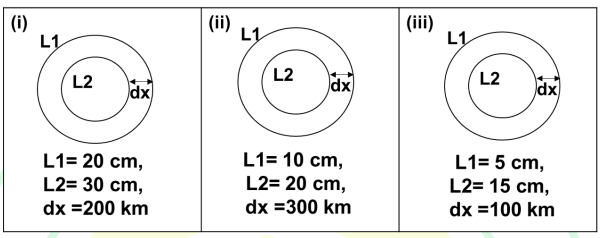
\includegraphics[width=0.5\columnwidth]{figs/fig34.png}
    \caption{}
    \label{fig:placeholder}
\end{figure}

Which one of the following orders is correct about the magnitudes of the geostrophic currents within the isolines?

\hfill[GATE XE 2025]

\begin{multicols}{2}
\begin{enumerate}
\item $(i) > (ii) > (iii)$
\item $(ii) > (iii) > (i)$
\item $(iii) > (i) > (ii)$
\item $(iii) > (ii) > (i)$
\end{enumerate}
\end{multicols}

\item The vertical (depth) profiles for three parameters P1, P2, and P3 in the northern Indian Ocean are given in the figure below. The values along the x-axis are the normalized values of the parameters and y-axis is the depth (m). Identify the parameters P1, P2, and P3 from the options given below.

\begin{figure}[H]
    \centering
    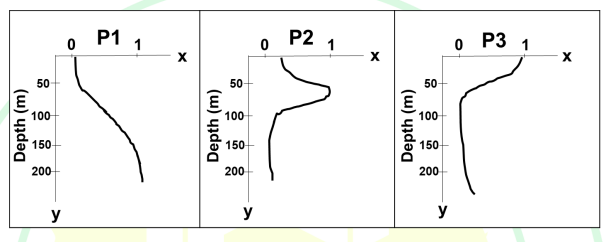
\includegraphics[width=0.5\columnwidth]{figs/fig35.png}
    \caption{}
    \label{fig:placeholder}
\end{figure}

\hfill[GATE XE 2025]

\begin{multicols}{2}
\begin{enumerate}
\item P1: Dissolved Oxygen; P2: Nitrate; P3: Chlorophyll
\item P1: Nitrate; P2: Chlorophyll; P3: Dissolved Oxygen
\item P1: Dissolved Oxygen; P2: Chlorophyll; P3: Nitrate
\item P1: Chlorophyll; P2: Nitrate; P3: Dissolved Oxygen
\end{enumerate}
\end{multicols}

\item The zonal gradient of meridional current and the meridional gradient of zonal current is $-0.3 \times 10^{-3} \; \text{s}^{-1}$
 and $0.3 \times 10^{-3} \; \text{s}^{-1}$
, respectively, at a location P (87 °E, 15 °N). Which one of the following best explains the nature of the flow?

\hfill[GATE XE 2025]

\begin{multicols}{2}
\begin{enumerate}
\item The flow is non-divergent in nature.
\item The flow is non-rotational in nature.
\item The flow is counter-clockwise in nature.
\item The flow is clockwise in nature.
\end{enumerate}
\end{multicols}

\item The north-Atlantic deep-water is associated with  \rule{3cm}{0.15mm}.

\hfill[GATE XE 2025]

\begin{multicols}{2}
\begin{enumerate}
\item low temperature and low salinity
\item high temperature and high salinity
\item high temperature and low salinity
\item low temperature and high salinity
\end{enumerate}
\end{multicols}

\item Which of the following is the correct form of the mass divergence form of the continuity equation for a compressible fluid?
[In the given equations, $\rho$ is the density and v the three dimensional velocity vector of the fluid.]

(i) \(\dfrac{\partial \rho}{\partial t} + \nabla \times (\rho \mathbf{v}) = 0\)

(ii) \(\dfrac{\partial \rho}{\partial t} + \nabla \cdot (\rho \mathbf{v}) = 0\)

(iii) \(\dfrac{\partial \mathbf{v}}{\partial t} + \rho \cdot \nabla \mathbf{v} = 0\)

(iv) \(\dfrac{\partial \rho}{\partial t} + \mathbf{v} \cdot \nabla \rho = 0\)

\hfill[GATE XE 2025]

\begin{multicols}{2}
\begin{enumerate}
\item (i) and (ii)
\item (ii)
\item (i) and (iv)
\item (iii)
\end{enumerate}
\end{multicols}

\item In the figures given below, L and H indicate low and high pressure centers, respectively; PGF, CoF and CeF indicate Pressure Gradient Force, Coriolis Force and Centrifugal Force, respectively; V is Velocity. [The arrows indicate only the directions but not the magnitudes of the forces and velocity.]
Which of the following is/are the correct representation(s) of the directions of various forces and velocity in the gradient wind balance in the northern hemisphere?

\begin{figure}[H]
    \centering
    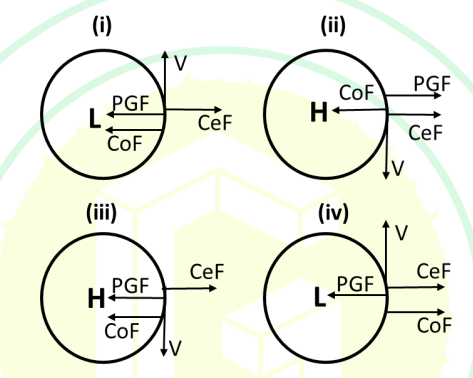
\includegraphics[width=0.5\columnwidth]{figs/fig36.png}
    \caption{}
    \label{fig:placeholder}
\end{figure}

\hfill[GATE XE 2025]

\begin{multicols}{2}
\begin{enumerate}
\item (i)
\item (ii)
\item (iii)
\item (iv)
\end{enumerate}
\end{multicols}

\item One kg of dry air at 15 °C is isothermally compressed to one-tenth of its initial volume. The work done on the system is \rule{3cm}{0.15mm} kJ. (Round off to the nearest integer.)
[Assume that the gas constant for dry air is $287 \times 10^{5}$
 J K-1 kg-1.]

\hfill[GATE XE 2025]

\item In hot weather, a human body cools by the evaporation of sweat from its skin. The amount of water that must evaporate to cool the body by 1 °C is \rule{3cm}{0.15mm} % of the body mass. (Round off to two decimal places.)
[Assume that latent heat of vaporization of water is $2.25 \times 10^{6}$
 J kg-1 and specific heat capacities of both human body and liquid water is $4.2 \times 10^{3}$
 J K-1 kg-1.]

\hfill[GATE XE 2025]

\item A floating hot air balloon with volume $1000 m^3$ and gross mass (excluding the air in the balloon) 100 kg is in hydrostatic balance where the external air temperature is 10\degree C and density is 1 kg m-3. The temperature of the air inside the balloon is \rule{3cm}{0.15mm} °C. (Round off to the nearest integer.)

\hfill[GATE XE 2025]

\item The solar constant for the Earth is 1368 W m-2. Consider the planet Jupiter whose mass is 320 times that of the Earth and distance from the Sun is 5.2 times that of the Earth. The solar constant for Jupiter is \rule{3cm}{0.15mm} W m-2. (Round off to the nearest integer.)

\hfill[GATE XE 2025]

\item A column of air mass extending from surface to a height of 10 km moving eastward along 30 °N strikes a north-south oriented mountain range. While crossing the mountain range, the air mass acquires a relative vorticity of $-3.65 × 10^-5 s^-1$ at the top. If the air mass maintains the same latitude and conserves potential vorticity, the height of the mountain range is \rule{3cm}{0.15mm} km. (Round off to the nearest integer.)
[Assume the angular velocity of the Earth is $7.3 × 10^-5 s^-1$ and initial relative vorticity is zero.]

\hfill[GATE XE 2025]

\item The Sea Surface Temperature, Air Temperature and 10 m Wind Speed at the locations P and Q are given in the table below. [Assume the density of air, specific heat capacity, and sensible heat transfer constant are the same at both locations.]

\begin{tabular}{|c|c|c|c|}
\hline
Location & Sea Surface temperature ($^{\circ}$C) & Air temperature ($^{\circ}$C) & Wind Speed at 10m (m s$^{-1}$) \\
\hline
P & 28 & 35 & 4 \\
\hline
Q & 30 & 32 & 7 \\
\hline
\end{tabular}

The sensible heat (SH) flux at the locations P and Q are SH\(_\text{P}\) and SH\(_\text{Q}\), respectively. The value of (SH\(_\text{P}\)/SH\(_\text{Q}\)) is \rule{3cm}{0.15mm}. (in integer)

\hfill[GATE XE 2025]

\end{enumerate}

\end{document}
